\documentclass[a4paper,fleqn]{cas-dc}
\usepackage[numbers,sort&compress]{natbib}
\usepackage{amsmath,amssymb}
\usepackage{booktabs}
\usepackage{graphicx}
\usepackage{algorithm}
\usepackage{algpseudocode}
\usepackage[figuresright]{rotating}

\graphicspath{{../output/figures/}}

\providecommand{\ktablecaption}{}

\begin{document}

% Page 1: Highlights
\noindent{\Large\bfseries Highlights}\par
\vspace{1.2em}
\noindent{\large\bfseries Multi-Task Particle Swarm Optimization with Knowledge-Guided Elite Refinement and Two-Phase Weight Scheduling for High-Dimensional Feature Selection}\par
\vspace{0.6em}
\noindent Anonymous Author\par
\vspace{1.5em}

\begin{itemize}\setlength{\itemsep}{10pt}
  \item Closed-loop knowledge-guided swarm learning framework for high-dimensional feature selection.
  \item MI initialization with adaptive re-initialization restores diversity and prevents search entrapment.
  \item Knowledge-guided elite refinement accumulates feature-importance signals with exponential decay.
  \item Two-phase weight scheduling temporally decouples feature compression from accuracy refinement.
  \item KDS-EL achieves 95.74\% accuracy with 87.8 selected features across 20 benchmark datasets.
\end{itemize}

\clearpage

\shorttitle{Multi-Task PSO with Knowledge-Guided Elite Refinement and Two-Phase Weight Scheduling}
\shortauthors{Anonymous Author}

\title[mode=title]{Multi-Task Particle Swarm Optimization with Knowledge-Guided Elite Refinement and Two-Phase Weight Scheduling for High-Dimensional Feature Selection}

\author[1]{Anonymous Author}
\cormark[1]
\ead{corresponding.author@example.com}
\address[1]{School of Computer Science, Anonymous University, Anonymous City, China}
\cortext[cor1]{Corresponding author}

\begin{abstract}
Feature selection in high-dimensional data remains a central challenge for evolutionary computation. Particle swarm optimization suffers from three structural deficiencies: random initialization provides insufficient guidance in sparse high-dimensional spaces, uniform feature perturbation fails to exploit cross-iteration feature-importance signals, and static objective preferences cannot adapt to different evolutionary phases. To address these limitations, we propose KDS-EL (Knowledge-Guided Dual-Phase Swarm Evolutionary Learning), a knowledge-guided evolutionary framework with a closed-loop feature-importance learning mechanism. First, to overcome inefficient initialization, we propose mutual-information-guided initialization with adaptive re-initialization, injecting prior knowledge and recovering population diversity when stagnation occurs. Second, to exploit discarded cross-iteration feature-importance signals, we propose a knowledge-guided elite refinement strategy that accumulates feature-importance knowledge and steers elite solutions toward historically effective features. Third, to align objective weights with search phases, we propose two-phase weight scheduling that emphasizes early dimensionality reduction and late-stage accuracy refinement. On 20 high-dimensional benchmarks, KDS-EL achieves the best classification performance among all competitors, with a mean accuracy of 0.9574 and only 87.8 selected features, outperforming the strongest single- and multi-objective competitors by +3.97 and +4.42 percentage points; Wilcoxon signed-rank tests with Holm--Bonferroni correction confirm statistically significant improvements over all 13 competitors.
\end{abstract}

\begin{keywords}
Feature selection \sep Particle swarm optimization \sep Mutual information \sep Knowledge-guided elite refinement \sep Two-phase weight scheduling
\end{keywords}

\maketitle

\section{Introduction}\label{sec:introduction}

High-dimensional data have emerged as a fundamental challenge in classification problems across diverse domains, including genomics, text mining, and computer vision. These datasets typically contain hundreds or even tens of thousands of features, while only a limited number of labeled samples are available, resulting in the well-known \(p \gg n\) scenario. Under such conditions, conventional learning algorithms often suffer from severe overfitting, increased computational complexity, and reduced interpretability due to the curse of dimensionality~\cite{lili2017,guyon2003}. Feature selection (FS) has therefore become an essential preprocessing technique that aims to identify a compact and informative subset of features while preserving classification performance. However, selecting an optimal feature subset remains highly challenging because the search space grows exponentially with the number of features \(D\), and the underlying subset-selection problem is NP-hard~\cite{liang2025}. Moreover, individual feature relevance measures are insufficient to characterize complex feature interactions and dependencies, which are often critical for achieving robust classification performance.

FS methods are generally categorized into filter, wrapper, and embedded approaches~\cite{kohavi1997,lili2017}. Filter methods rank features according to statistical criteria and offer high computational efficiency, but they usually evaluate features independently of the classifier and may overlook feature interactions relevant to classification. Embedded methods incorporate feature selection into the learning process, providing a compromise between selection efficiency and predictive performance; however, their effectiveness is often dependent on the characteristics of specific learning models. Wrapper methods directly optimize feature subsets according to classifier performance and can achieve competitive classification results, but the repeated model evaluations make them computationally expensive, especially in high-dimensional search spaces. To address the combinatorial complexity of wrapper-based FS, evolutionary computation has been extensively investigated as a promising optimization paradigm~\cite{liang2025,kennedy1995,shi1998,kennedy1997}. By maintaining a population of candidate solutions, evolutionary algorithms can perform global exploration of feature subsets without requiring gradient information. Among them, particle swarm optimization (PSO), genetic algorithms, and differential evolution have demonstrated promising results on high-dimensional FS tasks.

PSO has become one of the most widely adopted evolutionary algorithms for FS due to its simple structure, efficient information-sharing mechanism, and fast convergence. Nevertheless, conventional PSO-based FS methods still encounter three structural limitations when dealing with sparse and high-dimensional search spaces. First, random initialization distributes particles without prior guidance throughout the binary search space, whereas effective feature subsets usually occupy only a small region with limited active dimensions. Consequently, a considerable number of fitness evaluations may be wasted on redundant and suboptimal solutions before the swarm identifies promising search regions. Second, conventional uniform feature perturbation strategies treat all dimensions equally and neglect the feature-level improvement information accumulated during previous evaluations, preventing the search from exploiting historically informative features. Third, existing PSO-based FS methods typically employ fixed objective weights to balance classification error and feature subset size during the entire optimization process. However, the desired trade-off between feature reduction and accuracy refinement varies across search stages: aggressive sparsity enhancement is preferred in early exploration, whereas accurate decision boundary refinement becomes more important after a compact subset has been obtained.

Recent evolutionary FS studies have attempted to improve search performance through enhanced population initialization, adaptive evolutionary operators, and refined fitness evaluation strategies~\cite{wangjia2022,wang2022,xuezhang2024,wei2025}. Although these approaches have achieved promising results, they usually focus on isolated components of the optimization process and do not jointly address inefficient initialization, insufficient exploitation of accumulated feature knowledge, and inflexible objective weighting. Recently, multi-task PSO has emerged as an effective paradigm for high-dimensional FS with fixed-length binary representations. For instance, MEL~\cite{mel2024} adopts cooperative subpopulations and a fixed-length representation to efficiently handle feature spaces containing tens of thousands of dimensions. Despite its effectiveness, existing multi-task PSO-based FS frameworks still leave several challenges unresolved: the initial population is generally generated without sufficient feature-level prior knowledge, useful feature-importance information discovered during evolution is not explicitly retained and exploited, and the balance between classification performance and feature sparsity remains unchanged across different search stages.

To address these limitations, this paper proposes Knowledge-Guided Dual-Phase Swarm Evolutionary Learning (KDS-EL), a closed-loop framework that cohesively integrates domain prior injection, cross-iteration knowledge accumulation, and dynamic objective scheduling into a cooperative multi-task PSO backbone.

The main contributions of this paper are summarized as follows:
\begin{enumerate}
\item \textit{MI-Guided Initialization with Adaptive Re-initialization}: A hybrid seeding strategy that injects continuous feature-relevance priors into population construction to eliminate early-stage search waste, coupled with an adaptive re-initialization mechanism that restores swarm diversity upon evolutionary stagnation (Section~\ref{sec:mi}).
\item \textit{Knowledge-Guided Elite Refinement (KER)}: A targeted elite perturbation operator that dynamically harvests cross-iteration feature-importance feedback with exponential memory decay, directing elite solutions toward historically effective features within a strictly bounded evaluation overhead (Section~\ref{sec:ker}).
\item \textit{Two-Phase Weight Scheduling (TPS)}: A stage-aware objective scheduling mechanism that temporally decouples early aggressive feature pruning from late-stage accuracy refinement, overcoming the rigidity of static weighting (Section~\ref{sec:twophase}).
\item \textit{Comprehensive Empirical Validation}: Extensive evaluations across 20 high-dimensional benchmark datasets (spanning 500 to 54{,}675 features) against state-of-the-art single-objective competitors and precursor frameworks, rigorously validated through non-parametric statistical testing, component contribution analysis, and parametric sensitivity investigations (Section~\ref{sec:results}).
\end{enumerate}

Extensive experiments demonstrate that KDS-EL achieves the highest classification performance, obtaining an average classification accuracy of 0.9574 with only 87.8 selected features, corresponding to an average feature selection ratio of merely 1.1\%. Compared with recent top-tier competitor bIRIME~\cite{su2024} and established competitor FWPSO~\cite{wangjia2022}, KDS-EL improves classification accuracy by 1.20 and 3.97 percentage points, while reducing the selected feature count by 78.5\% and 91.8\%, respectively. Furthermore, KDS-EL achieves a 3.4$\times$ speedup over the foundational multi-task precursor MEL~\cite{mel2024}, reducing average runtime from 175.0\,s to 51.3\,s. Pairwise Wilcoxon signed-rank tests with Holm--Bonferroni step-down correction confirm that the performance advantages are statistically significant over all 11 comparison algorithms and ablative variants.

The remainder of this paper is organized as follows. Section~\ref{sec:related} formulates the feature selection optimization problem and reviews related literature and background concepts. Section~\ref{sec:proposed} presents the proposed KDS-EL framework and formulates its three constituent mechanisms in detail. Section~\ref{sec:results} presents comprehensive experimental results, statistical tests, component contribution analysis, and parameter sensitivity investigations. Finally, Section~\ref{sec:conclusion} concludes the paper and discusses prospective research directions.

\section{Related Work}\label{sec:related}

\subsection{Feature Selection Paradigms}

Feature selection is a fundamental pre-processing step in high-dimensional data analysis, aiming to identify a minimal subset of relevant features that preserves or improves classification performance while reducing computational cost and enhancing interpretability \cite{lili2017,guyon2003}. Methods fall broadly into three paradigms: filter, wrapper, and embedded.

Filter methods evaluate features independently of any learning algorithm, relying on intrinsic data properties such as variance, correlation, or eigenvector centrality \cite{kramer1991,roffo2016}. Representative techniques include the minimum Redundancy Maximum Relevance (mRMR) criterion \cite{peng2005} and the Fast Correlation-Based Filter (FCBF) \cite{yu2003}. These methods are computationally efficient and scale readily to high-dimensional settings, yet they disregard feature interactions and may retain redundant subsets under strong inter-feature correlation.

Wrapper methods treat feature selection as a search problem, evaluating candidate subsets by the predictive performance of a specific classifier \cite{kohavi1997}. Hybrid genetic algorithms \cite{oh2004} and other meta-heuristic wrappers can capture complex feature interdependencies, but their computational cost grows rapidly with dimensionality, as each candidate subset requires a full classifier training-and-evaluation cycle.

Embedded methods integrate feature selection into model training. Lasso and its bootstrapped variant Bolasso \cite{bach2008} enforce sparsity through $L_1$ regularization; gradient-boosting-based approaches such as FS-GBDT \cite{zhang2021fsgbdt} leverage tree-split importance; and hybrid algorithms like ILRC \cite{yu2021ilrc} combine regularization with clustering. Embedded methods offer a favorable speed--accuracy trade-off, but their feature rankings are tied to specific model assumptions.

At high dimensionality, each paradigm faces distinct structural bottlenecks: filters are fast but oblivious to feature interactions, wrappers are accurate but face a search space that grows exponentially with dimension, and embedded methods depend on model-specific regularization biases. These complementary weaknesses motivate evolutionary computation, which decouples the search mechanism from the evaluation metric and navigates the exploration--exploitation trade-off through population-based global search.

\subsection{Single-Objective Evolutionary Feature Selection}

Evolutionary algorithms have been extensively applied to feature selection for their population-based global search and gradient-free nature. Early work adapted classical meta-heuristics---binary PSO (BPSO) \cite{kennedy1997}, ant colony optimization (ACO) \cite{aghdam2009}, artificial bee colony (ABC) \cite{karaboga2007}, and genetic algorithms with support vector machines (GA-SVM) \cite{huang2006}---to the binary subset selection problem, establishing the template of a population of candidate subsets evolving under selection, crossover, and mutation guided by a scalar fitness function.

Because standard evolutionary operators degrade at high dimensionality, specialized single-objective methods have been developed: self-adaptive PSO adjusting swarm size and mutation rate \cite{xue2019}, progressively refined PSO alternating between coarse- and fine-grained search \cite{prasad2015}, and problem-specific heuristics---FWPSO~\cite{wangjia2022}, which biases velocity updates with per-feature importance; SaWDE~\cite{wang2022} with adaptive weighting; IGPSO~\cite{xuezhang2024}, which estimates relevance via a multi-layer perceptron; and PSO-CSM~\cite{wei2025} integrating multiple evaluation criteria. Learning-based control and space decomposition are also explored: reinforcement-learning-aided PSO~\cite{weil2025} and divide-and-conquer search~\cite{chen2025}. These methods refine search operators but do not systematically exploit accumulated feature-importance knowledge harvested from the search itself.

\subsection{Multi-Objective Evolutionary Feature Selection}

Multi-objective formulations treat classification accuracy and feature count as competing objectives, producing a Pareto front of non-dominated solutions. Xue et al. \cite{xue2012mopso} pioneered multi-objective PSO for feature selection, showing that jointly optimizing accuracy and subset size yields more diverse and informative solutions than scalarized approaches. Hu et al. \cite{hu2020} extended this framework with fuzzy cost functions for imbalanced classification.

The multi-objective evolutionary algorithm (MOEA) family provides several architectures for this problem. NSGA-II-FS \cite{deb2002} uses non-dominated sorting and crowding distance to maintain Pareto-front diversity. MOEA/D-FS \cite{zhang2007} decomposes the problem into scalar subproblems solved cooperatively. MOPSO-FS \cite{coello2004} extends single-objective PSO with an external archive and Pareto-dominance-based leader selection. For high-dimensional data, Cheng et al. \cite{cheng2023} proposed a variable-granularity search method (VGS-MOEA) that transitions from coarse to fine-grained search, and Hancer et al. \cite{hancer2023} combined evolutionary search with filter-based ranking under both single- and multi-objective settings.

Despite their conceptual advantages, MOFS methods incur substantial overhead: maintaining an external archive, non-dominated sorting, and Pareto-front management all cost significant time (in our experiments, over 110 seconds on average). Moreover, under fixed-length binary encoding at high dimensionality, the Pareto front expands combinatorially and convergence slows, limiting scalability at gene-expression scale.

\subsection{Evolutionary Multi-Task Learning}

Evolutionary multi-task learning (EMTL) solves multiple related tasks jointly, with knowledge transfer accelerating convergence. Zhang and Yang \cite{zhang2021mtl} surveyed its foundations, and several instantiations target feature selection: a minion-based multitasking framework \cite{zhang2021minion}, PSO-based multitasking for high-dimensional classification \cite{chen2020emfs,chen2021emfs}, multitask bee colony optimization for hyperspectral band selection \cite{he2022}, and multitasking for large-scale multi-objective optimization \cite{liu2022}.

Of particular relevance, Wang et al. \cite{mel2024} proposed MEL (Multi-task Evolutionary Learning), a dual-swarm multi-task PSO in which one swarm optimizes binary feature subsets while a second learns continuous feature weights, with the swarms cooperating through cross-task knowledge transfer. MEL was selected as the backbone for three reasons: its fixed-length encoding is efficient at high dimensionality and naturally compatible with incremental augmentation; its dual-space cooperation provides a built-in mechanism for capturing feature relevance signals; and it has demonstrated strong performance on gene-expression benchmarks.

Nevertheless, MEL exhibits three structural limitations. Its population is initialized entirely at random, wasting search budget in the sparse high-dimensional space. Its operators---velocity update and mutation---are uniform and stochastic, never incorporating cross-iteration knowledge about which features have proven beneficial. And its dual-objective weights remain fixed throughout search, imposing a rigid schedule that cannot adapt to the natural phasing of feature selection, where early iterations benefit from aggressive compression and later iterations demand fine-grained accuracy refinement.

\subsection{Gene-Expression Feature Selection}

High-dimensional gene expression data present a particularly challenging testbed: the number of features routinely exceeds the number of samples by three to four orders of magnitude---a ``small $N$, large $D$'' regime where conventional statistical methods break down and overfitting is pervasive \cite{bermingham2015,phuong2005}. Representative applications include cancer staging \cite{saghapour2017}, Alzheimer's classification from neuroimaging features \cite{zhang2015eigenbrain}, biomarker gene identification \cite{wangjia2022}, and multi-cancer risk module discovery \cite{zhang2021fsgbdt,yu2021ilrc}.

Two structural properties amplify the difficulty. First, feature redundancy is exceptionally high: co-regulated genes exhibit correlated expression, so distinct subsets frequently yield near-identical accuracy. Second, a non-trivial fraction of gene datasets reach accuracy ceilings---exceeding 0.998 under multiple methods---rendering accuracy alone insufficient to distinguish algorithmic quality; on these datasets the selected feature count becomes the primary discriminatory metric. Evaluation must therefore jointly consider classification accuracy and subset compactness.

Recent methodological development in this area is extensive; surveys of evolutionary computation for biomarker identification in complex diseases \cite{liang2025} and instance-selection-assisted evolutionary feature selection \cite{xia2026} both target the small-sample, ultra-high-dimensional regime central to gene-expression analysis.

\subsection{Positioning of KDS-EL}

KDS-EL builds upon the multi-task PSO backbone of MEL, adding three mechanisms that each target one structural limitation: MI-guided initialization with adaptive re-initialization addresses the cold-start problem; the KER strategy injects cross-iteration feature importance into elite refinement at no additional cost; and Two-Phase Weight Scheduling replaces static weights with a compression-then-refinement schedule. These mechanisms preserve the fixed-length encoding that makes the backbone suitable for high-dimensional applications.

\section{Preliminaries}\label{sec:preliminaries}

Particle swarm optimization (PSO), introduced by Kennedy and Eberhart~\cite{kennedy1995}, maintains a population of candidate solutions that traverse the search space guided by personal and collective historical experience. Each particle $i$ holds a position $\mathbf{x}_i \in \mathbb{R}^D$ and a velocity $\mathbf{v}_i \in \mathbb{R}^D$, updated at iteration $t$ according to
\begin{equation}
\mathbf{v}_i^{(t+1)} = \omega \mathbf{v}_i^{(t)} + c_1 r_1 (\mathbf{p}_{\text{best},i} - \mathbf{x}_i^{(t)}) + c_2 r_2 (\mathbf{g}_{\text{best}} - \mathbf{x}_i^{(t)}),
\label{eq:pso_velocity}
\end{equation}
where $\omega$ is the inertia weight introduced by Shi and Eberhart~\cite{shi1998}, $c_1, c_2$ are acceleration coefficients, $r_1, r_2 \sim \mathcal{U}(0,1)$ are independent random scalars, and $\mathbf{p}_{\text{best},i}$ and $\mathbf{g}_{\text{best}}$ denote the personal and global best positions, respectively. For binary feature selection, the continuous-valued position is mapped to a binary mask through a sigmoid transfer function \cite{kennedy1997}:
\begin{equation}
S(v_{i,d}) = \frac{1}{1 + e^{-v_{i,d}}}, \qquad
x_{i,d} = \begin{cases} 1 & \text{if } \mathrm{rand}() < S(v_{i,d}), \\ 0 & \text{otherwise},
\end{cases}
\label{eq:bpsosigmoid}
\end{equation}
with a threshold of 0.6, as adopted throughout this paper. In the $p \gg n$ regime, standard BPSO converges slowly and tends toward premature stagnation, as the velocity update provides no domain-grounded gradient toward sparse, high-accuracy regions.

MEL (Multi-task Evolutionary Learning) \cite{mel2024} recasts high-dimensional FS as a dual-task problem solved by two co-evolving PSO swarms: one operates on binary feature-subset vectors $\mathbf{x} \in \{0,1\}^D$ encoding hard selection decisions, the other on continuous feature-weight vectors $\mathbf{w} \in [0,1]^D$ encoding importance scores. The swarms exchange knowledge through periodic elite migration---the best individuals of each swarm replace the weakest of the other---coupling discrete cardinality control with continuous importance refinement. Readers are referred to \cite{mel2024} for full details. KDS-EL builds on three interfaces exposed by this framework: the $D$-dimensional binary position encoding shared by all components of Section~\ref{sec:proposed}; the per-generation selection of $k$ elite particles by scalar fitness, which the KER strategy extends with knowledge-guided perturbation; and the fitness function, a weighted sum of classification error and subset sparsity:
\begin{equation}
f(\mathbf{x}) = w_s^{(0)} \cdot \bigl(1 - \mathrm{Acc}(\mathbf{x})\bigr) + w_s^{(1)} \cdot \frac{\|\mathbf{x}\|_0}{D},
\label{eq:fitness_mel}
\end{equation}
where $\mathrm{Acc}(\mathbf{x})$ is the $k$-nearest neighbor accuracy on the selected features, $\|\mathbf{x}\|_0$ is the number of selected features, and $\mathbf{w}_s = (w_s^{(0)}, w_s^{(1)})$ is a static weight vector. In MEL, $\mathbf{w}_s$ remains constant throughout search---a design Section~\ref{sec:proposed} replaces with Two-Phase Weight Scheduling. MEL's per-generation cost is dominated by both swarms' fitness evaluations, each requiring classifier training and cross-validation, giving overall complexity $O(T \cdot N \cdot T_{\mathrm{eval}})$.

\section{Proposed KDS-EL Algorithm}\label{sec:proposed}

In this section, we present the comprehensive architectural design, mathematical formulation, and algorithmic execution of the proposed \textbf{Knowledge-Guided Dual-Phase Swarm Evolutionary Learning (KDS-EL)} algorithm. KDS-EL is designed specifically to overcome three fundamental structural deficiencies of conventional particle swarm optimization in ultra-high-dimensional feature selection: (i) the search inefficiency and wasted evaluation budget caused by uniform random initialization in sparse feature spaces, (ii) the loss of historical cross-iteration feature-importance signals due to memoryless random perturbation, and (iii) the inability of static objective weighting to adapt to the divergent requirements of coarse feature reduction versus fine-grained accuracy refinement.

\subsection{Overall Algorithmic Architecture}

\begin{figure}[!htb]
\centering
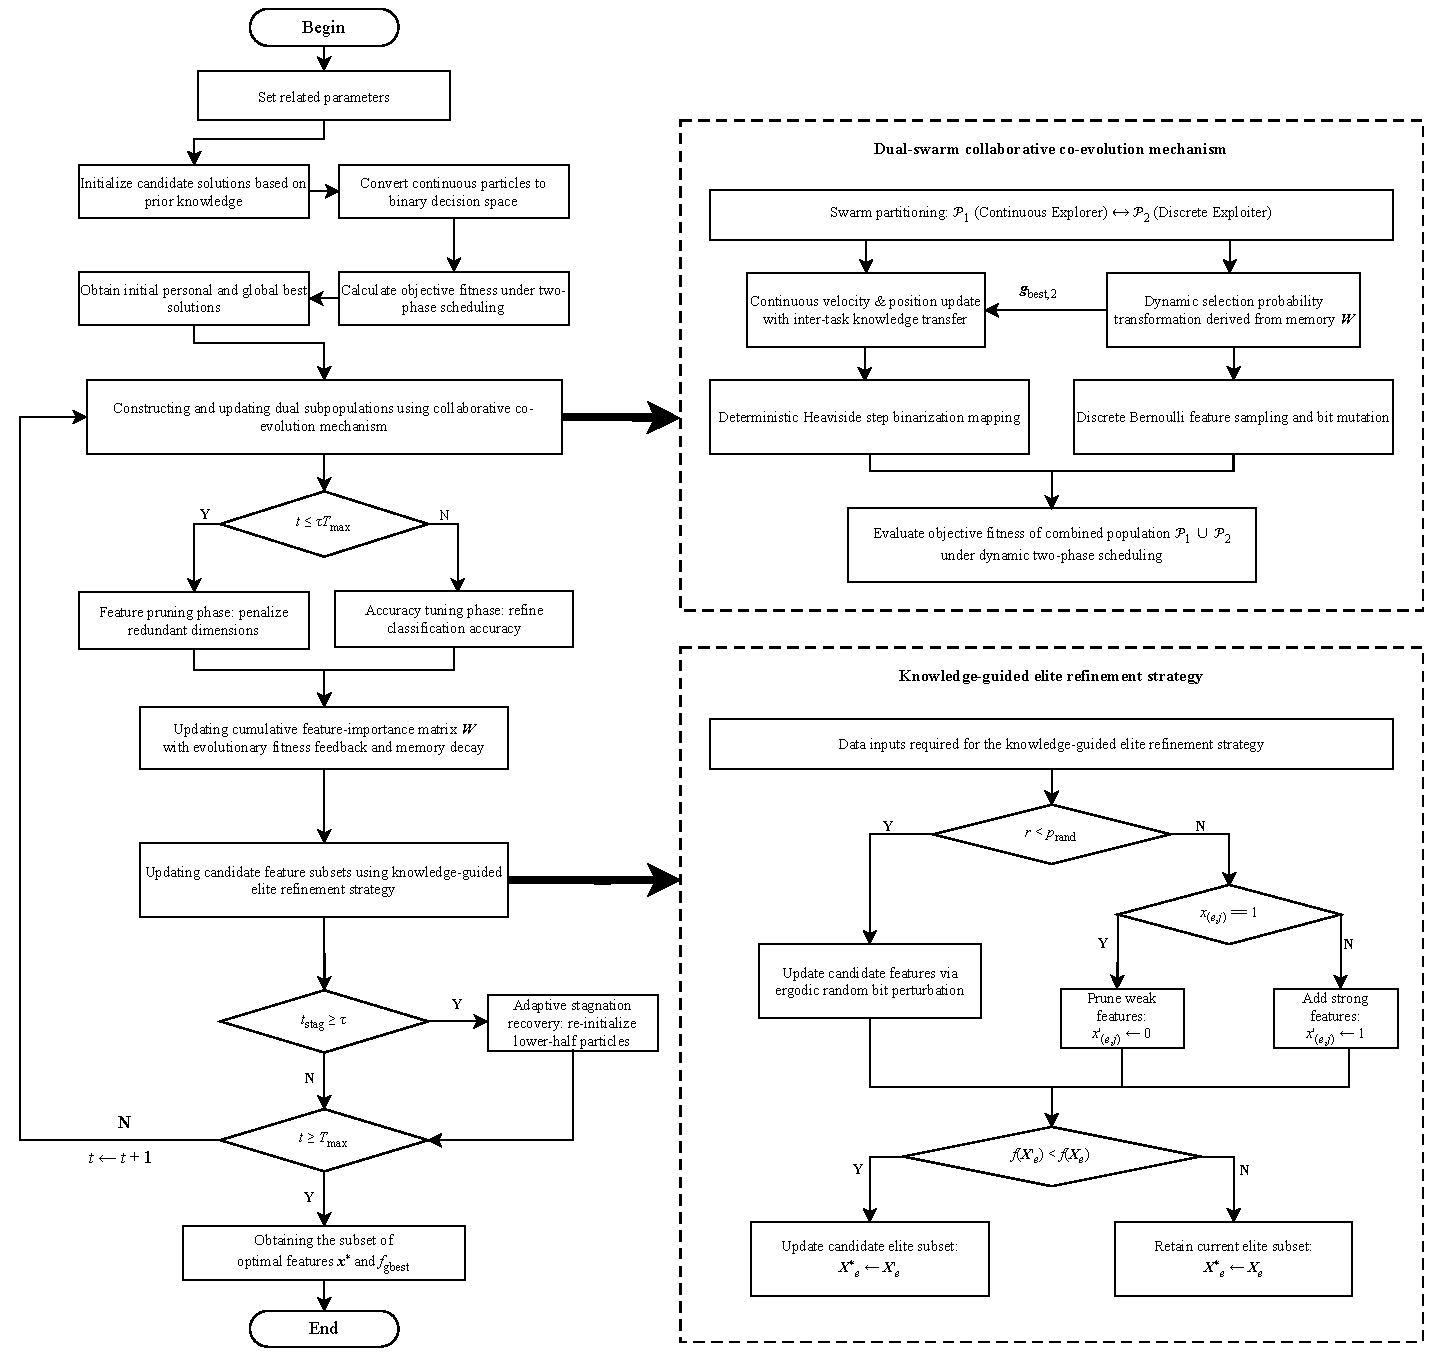
\includegraphics[width=\linewidth]{F1_architecture_journal.pdf}
\caption{Overall architectural pipeline of KDS-EL: high-dimensional data undergo filter-based mutual information ranking, dual-subpopulation initialization with Gaussian perturbation, two-phase dynamic objective weight scheduling, cross-iteration cumulative feature-importance matrix accumulation with exponential decay, and knowledge-guided elite refinement with 1-to-1 in-place replacement.}
\label{F1}
\end{figure}

The macroscopic architecture of KDS-EL is illustrated in Fig.~\ref{F1}. Built upon a cooperative multi-task dual-subpopulation backbone~\cite{mel2024}, KDS-EL divides a population of $N=20$ binary particles into two collaborative subpopulations of equal size ($N_1 = N_2 = 10$). Subpopulation~1 ($\mathcal{P}_1$) executes standard continuous-space PSO velocity-position updates with an inter-task knowledge transfer channel directing particles toward the historical global best of Subpopulation~2. Subpopulation~2 ($\mathcal{P}_2$) performs probability-driven feature sampling guided by the population's accumulated feature-importance landscape.

The optimization process operates in a closed loop through four tightly coupled functional stages:
\begin{enumerate}
    \item \textbf{Filter-Level Quality Bootstrapping (Offline)}: Mutual information (MI) between each feature and class labels is computed once prior to evolution, establishing a normalized baseline relevance vector $\mathbf{m} \in [0, 1]^D$.
    \item \textbf{Knowledge-Informed Hybrid Seeding}: An initial population of $N$ particles is generated by blending Gaussian-perturbed MI seeds with uniform random particles at a ratio of $\mathrm{MI\_init\_ratio}=0.50$, followed by Heaviside step binarization with threshold $\theta=0.60$.
    \item \textbf{Dynamic Two-Phase Evolutionary Loop}: Across $T=100$ iterations, the objective weights $\mathbf{w}(t) = [w_a(t), w_f(t)]$ dynamically transition from aggressive feature pruning ($\mathbf{w}_1 = [0.70, 0.30]$ for $t \le 0.7T$) to accuracy-oriented refinement ($\mathbf{w}_2 = [0.95, 0.05]$ for $t > 0.7T$).
    \item \textbf{Accumulative Knowledge Harvesting and Elite Refinement}: Fitness improvements during evaluation are harvested into a continuous feature-importance matrix $W \in \mathbb{R}^D$, discounted by an exponential forgetting factor $\gamma=0.99$. The top $\mathrm{elite\_k}=3$ elite individuals are refined via the Knowledge-guided Elite Refinement (KER) operator and admitted via 1-to-1 in-place replacement. An adaptive re-initialization mechanism monitors stagnation and re-seeds the lower half of the population if global-best fitness stalls for $\mathrm{stall\_patience}=20$ generations.
\end{enumerate}

\subsection{MI-Prior Seeding and Adaptive Re-injection Strategy}\label{sec:mi}

\subsubsection{Deficiency Analysis and Design Rationale}

Standard binary meta-heuristics universally initialize particle positions via uniform random sampling over $[0, 1]^D$. In an ultra-high-dimensional feature space where $D \gg 10^3$, uniform random initialization produces candidate solutions where approximately $50\%$ of all features are active ($\|\mathbf{x}\|_0 \approx D/2$). However, for biomedical classification problems, true informative biomarker subsets are notoriously sparse, typically comprising fewer than $100$ genes ($\|\mathbf{x}^{\star}\|_0 \ll 0.01 D$). Consequently, random initialization forces the swarm into dense, highly redundant, and noisy search basins, squandering a major fraction of the computational evaluation budget simply attempting to discard thousands of irrelevant features.

To resolve this initial cold-start inefficiency, KDS-EL establishes a filter-wrapper hybrid seeding strategy that injects prior feature-relevance knowledge into the swarm origin while preserving sufficient stochastic diversity.

\subsubsection{Mathematical Formulation of MI Seeding}

Let $\mathcal{D} = \{(\mathbf{f}_i, y_i)\}_{i=1}^{N_{\mathrm{samp}}}$ denote the training set with $D$-dimensional feature vectors $\mathbf{f}_i$ and class labels $y_i \in \{1, \ldots, C\}$. The mutual information $I(f_j; Y)$ between the $j$-th feature $f_j$ and the label $Y$ is defined as:
\begin{equation}
I(f_j; Y) = \sum_{v \in \mathrm{Val}(f_j)} \sum_{c = 1}^C P(f_j = v, Y = c) \log_2 \frac{P(f_j = v, Y = c)}{P(f_j = v) P(Y = c)}.
\label{eq:mi_def}
\end{equation}
The continuous feature values are discretized into equal-frequency bins to estimate probability distributions. The raw MI scores $\{I(f_j; Y)\}_{j=1}^D$ are normalized into a baseline relevance vector $\mathbf{m} \in [0, 1]^D$:
\begin{equation}
m_j = \frac{I(f_j; Y) - \min_{1 \le k \le D} I(f_k; Y)}{\max_{1 \le k \le D} I(f_k; Y) - \min_{1 \le k \le D} I(f_k; Y) + \epsilon},
\label{eq:mi_norm}
\end{equation}
where $\epsilon = 10^{-12}$ prevents division by zero.

\begin{figure*}[!htb]
\centering
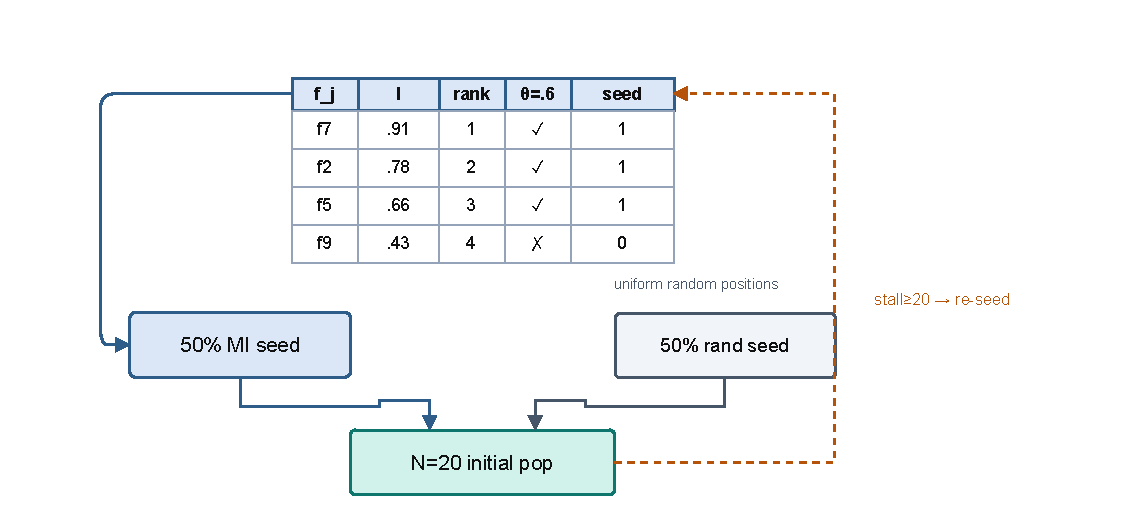
\includegraphics[width=0.96\linewidth]{F2_mi_initialization_journal.pdf}
\caption{Operational mechanism of MI-Prior Seeding and Adaptive Re-injection: mutual information $I(f_j; \mathbf{Y})$ extracts continuous feature--target dependency to construct a normalized prior vector $\widetilde{\mathbf{m}} \in [0, 1]^D$, which biases $50\%$ of initial particles with Gaussian perturbation while the remaining $50\%$ undergo uniform random exploration; when evolutionary search encounters stagnation ($\mathrm{stall} \ge 20$), the MI prior is adaptively re-injected into inferior particles to restore search vitality.}
\label{F2}
\end{figure*}

To prevent population homogenization while guiding search toward informative dimensions, the initial population is split into two halves based on $\rho = \mathrm{MI\_init\_ratio} = 0.50$:
\begin{equation}
\mathbf{p}_i = \begin{cases}
\mathrm{clip}\bigl(\mathbf{m} + \boldsymbol{\varepsilon}_i, \; 0, \; 1\bigr), \quad \boldsymbol{\varepsilon}_i \sim \mathcal{N}(\mathbf{0}, \sigma^2 I_D), & \text{for } 1 \le i \le \rho N,\\[4pt]
\mathbf{u}_i, \quad \mathbf{u}_i \sim \mathcal{U}(0, 1)^D, & \text{for } \rho N < i \le N,
\end{cases}
\label{eq:mi_seeding}
\end{equation}
where $\sigma = 0.10$ represents the Gaussian noise perturbation scale and $\mathrm{clip}(z, 0, 1) = \max(0, \min(1, z))$.

Continuous positions $\mathbf{p}_i = [p_{i,1}, \ldots, p_{i,D}]$ are mapped into binary feature selection vectors $\mathbf{x}_i \in \{0, 1\}^D$ using a strict Heaviside step binarization with threshold $\theta = 0.60$:
\begin{equation}
x_{i,j} = \begin{cases}
1, & \text{if } p_{i,j} \ge \theta,\\[2pt]
0, & \text{if } p_{i,j} < \theta.
\end{cases}
\label{eq:binarize}
\end{equation}
Because $\theta = 0.60 > 0.50$, only features possessing above-average mutual information are initialized as active, naturally yielding a sparse initial configuration ($\|\mathbf{x}_i\|_0 \approx 0.15 D \sim 0.30 D$) that accelerates early convergence. Algorithm~\ref{alg:mi_init} specifies the hybrid initialization procedure.

\begin{algorithm}[!htb]
\caption{MI-Guided Population Initialization}
\label{alg:mi_init}
\begin{algorithmic}[1]
\Require Normalized MI score vector $\mathbf{m} \in [0, 1]^D$, population size $N=20$, seeding ratio $\rho=0.50$, threshold $\theta=0.60$, noise scale $\sigma=0.10$
\Ensure Hybrid binary initial population $\mathcal{P} = \{\mathbf{x}_i\}_{i=1}^N$ and continuous positions $\{\mathbf{p}_i\}_{i=1}^N$
\For{$i = 1$ \textbf{to} $N$}
    \If{$i \le \lfloor \rho N \rfloor$}
        \State Sample perturbation $\boldsymbol{\varepsilon}_i \sim \mathcal{N}(\mathbf{0}, \sigma^2 I_D)$
        \State $\mathbf{p}_i \leftarrow \max\bigl(\mathbf{0}, \min(\mathbf{1}, \mathbf{m} + \boldsymbol{\varepsilon}_i)\bigr)$ \Comment{Knowledge-guided continuous seed}
    \Else
        \State Sample continuous position $\mathbf{p}_i \sim \mathcal{U}(0, 1)^D$ \Comment{Random exploratory seed}
    \EndIf
    \For{$j = 1$ \textbf{to} $D$}
        \State $x_{i,j} \leftarrow \mathbb{I}(p_{i,j} \ge \theta)$ \Comment{Thresholded binarization \eqref{eq:binarize}}
    \EndFor
\EndFor
\State \Return Binary population $\{\mathbf{x}_i\}_{i=1}^N$ and continuous positions $\{\mathbf{p}_i\}_{i=1}^N$
\end{algorithmic}
\end{algorithm}

\subsubsection{Adaptive Stagnation Re-initialization}

High-dimensional multimodal search landscapes frequently cause swarm particles to become trapped in suboptimal local attractors. When the global-best fitness $f_{\mathrm{gbest}}$ fails to improve for $\tau = \mathrm{stall\_patience} = 20$ consecutive iterations, an adaptive re-initialization routine is triggered:
\begin{enumerate}
    \item The population is sorted in ascending order of personal-best fitness $f_i^{\mathrm{pbest}}$.
    \item The superior half ($\{i \mid \mathrm{rank}(i) \le N/2\}$) is preserved to safeguard historical elite trajectories.
    \item The inferior half ($\{i \mid \mathrm{rank}(i) > N/2\}$) is fully refreshed using the Gaussian-perturbed MI distribution:
    \begin{equation}
    \mathbf{p}_i \leftarrow \mathrm{clip}\bigl(\mathbf{m} + \boldsymbol{\varepsilon}_i, \; 0, \; 1\bigr), \quad x_{i,j} \leftarrow \mathbb{I}(p_{i,j} \ge \theta).
    \label{eq:reinit_formula}
    \end{equation}
    \item The refreshed particles are re-evaluated under the current objective weights, and the stagnation counter is reset to zero.
\end{enumerate}
This restores diversity within a high-potential subspace without completely discarding established elite knowledge, as formalized in Algorithm~\ref{alg:mi_reinit}.

\begin{algorithm}[!htb]
\caption{Adaptive Stagnation Re-initialization}
\label{alg:mi_reinit}
\begin{algorithmic}[1]
\Require Population $\{\mathbf{x}_i, \mathbf{p}_i\}_{i=1}^N$, personal bests $\{\mathbf{p}_{\mathrm{best},i}, f_i^{\mathrm{pbest}}\}_{i=1}^N$, MI vector $\mathbf{m}$, threshold $\theta=0.60$, noise scale $\sigma=0.10$, objective weights $\mathbf{w}(t)$
\Ensure Refreshed population $\mathcal{P}$ with restored swarm diversity
\State Sort population indices $\pi$ such that $f_{\pi(1)}^{\mathrm{pbest}} \le f_{\pi(2)}^{\mathrm{pbest}} \le \cdots \le f_{\pi(N)}^{\mathrm{pbest}}$
\For{$k = \lfloor N/2 \rfloor + 1$ \textbf{to} $N$}
    \State $i \leftarrow \pi(k)$ \Comment{Target inferior particle}
    \State Sample perturbation $\boldsymbol{\varepsilon}_i \sim \mathcal{N}(\mathbf{0}, \sigma^2 I_D)$
    \State $\mathbf{p}_i \leftarrow \max\bigl(\mathbf{0}, \min(\mathbf{1}, \mathbf{m} + \boldsymbol{\varepsilon}_i)\bigr)$
    \State $x_{i,j} \leftarrow \mathbb{I}(p_{i,j} \ge \theta), \quad \forall j \in \{1, \ldots, D\}$
    \State Evaluate fitness $f_i \leftarrow f(\mathbf{x}_i, \mathbf{w}(t))$ using \eqref{eq:fitness}
    \State $\mathbf{p}_{\mathrm{best},i} \leftarrow \mathbf{x}_i, \quad f_i^{\mathrm{pbest}} \leftarrow f_i$
\EndFor
\State \Return Updated population and personal bests
\end{algorithmic}
\end{algorithm}

\subsection{Cumulative Feature-Importance Matrix with Exponential Memory Decay}\label{sec:importance}

\subsubsection{Deficiency Analysis and Design Rationale}

Standard PSO operators update particle trajectories purely based on instantaneous personal best ($\mathbf{p}_{\mathrm{best}}$) and global best ($\mathbf{g}_{\mathrm{best}}$) coordinates. Across consecutive evolutionary cycles, thousands of candidate subset evaluations are performed, generating abundant empirical evidence regarding which specific feature additions or deletions consistently enhance classification performance. Standard meta-heuristics completely discard this trial-and-error feedback upon the conclusion of each generation, suffering from severe evolutionary memory loss.

To capture and retain this cross-iteration evolutionary feedback, KDS-EL maintains a global continuous \textbf{Cumulative Feature-Importance Matrix} $W \in \mathbb{R}^D$, initialized to the zero vector $\mathbf{0}$.

\subsubsection{Differential Feedback Update and Exponential Forgetting}

At generation $t$, whenever a newly evaluated particle $\mathbf{x}_i^{(t)}$ achieves a strict fitness improvement over its historical personal best ($f_i^{(t)} < f_i^{\mathrm{pbest}}$), we extract the differential feature subset $\mathcal{C}_i^{(t)}$ containing features whose selection status changed:
\begin{equation}
\mathcal{C}_i^{(t)} = \bigl\{j \in \{1, \ldots, D\} \;\big|\; x_{i,j}^{(t)} \neq p_{\mathrm{best},i,j}\bigr\}.
\label{eq:changed_features}
\end{equation}
The magnitude of fitness improvement is quantified as:
\begin{equation}
\delta_i^{(t)} = f_i^{\mathrm{pbest}} - f_i^{(t)} > 0.
\label{eq:delta_fitness}
\end{equation}
Each changed feature $j \in \mathcal{C}_i^{(t)}$ receives a directional reward proportional to $\delta_i^{(t)}$:
\begin{equation}
W_j \leftarrow W_j + \delta_i^{(t)} \cdot (2 x_{i,j}^{(t)} - 1), \quad \forall j \in \mathcal{C}_i^{(t)},
\label{eq:importance_update}
\end{equation}
where $(2 x_{i,j}^{(t)} - 1) = +1$ if feature $j$ was newly activated (rewarding beneficial inclusion) and $-1$ if feature $j$ was deactivated (rewarding beneficial elimination). Features whose status remained unchanged, as well as non-improving particles ($\delta_i^{(t)} \le 0$), exert zero impact on $W$.

To prevent early-discovered features from dominating the matrix indefinitely and to allow the algorithm to forget stale historical correlations as the search shifts toward fine-grained subspaces, an exponential memory decay is applied to the entire matrix at the conclusion of each generation:
\begin{equation}
W \leftarrow \gamma \cdot W, \quad \text{where } \gamma = 0.99.
\label{eq:decay}
\end{equation}

\subsubsection{Theoretical Function of the Forgetting Factor $\gamma$}

The exponential decay factor $\gamma = 0.99$ fulfills two indispensable theoretical roles:
\begin{itemize}
    \item \textbf{Dynamic Rank Adaptation}: As the search progresses from coarse feature elimination to localized accuracy refinement, features that were critical in early generations may become redundant. The decay factor ensures that unless a feature repeatedly contributes to fitness improvements in recent generations, its cumulative score exponentially depreciates as $\gamma^k$, allowing newly discovered interactive features to rise in rank.
    \item \textbf{Score Saturation Prevention}: Without decay ($\gamma = 1.00$), cumulative importance values would grow monotonically unbounded ($W_j \to \infty$), causing the relative score distribution to saturate and destroying the sensitivity of downstream elite refinement operators.
\end{itemize}
Algorithm~\ref{alg:importance_update} outlines the per-generation importance harvesting and discounting procedure.

\begin{algorithm}[!htb]
\caption{Feature-Importance Matrix Update and Decay}
\label{alg:importance_update}
\begin{algorithmic}[1]
\Require Population candidates $\{\mathbf{x}_i\}_{i=1}^N$, personal bests $\{\mathbf{p}_{\mathrm{best},i}, f_i^{\mathrm{pbest}}\}_{i=1}^N$, candidate fitness $\{f_i\}_{i=1}^N$, current importance matrix $W \in \mathbb{R}^D$, decay factor $\gamma=0.99$
\Ensure Discounted cumulative feature-importance matrix $W$
\For{$i = 1$ \textbf{to} $N$}
    \If{$f_i < f_i^{\mathrm{pbest}}$}
        \State Compute improvement magnitude $\delta_i \leftarrow f_i^{\mathrm{pbest}} - f_i$
        \For{$j = 1$ \textbf{to} $D$}
            \If{$x_{i,j} \neq p_{\mathrm{best},i,j}$}
                \State $W_j \leftarrow W_j + \delta_i \cdot (2 x_{i,j} - 1)$ \Comment{Directional reward \eqref{eq:importance_update}}
            \EndIf
        \EndFor
    \EndIf
\EndFor
\State $W \leftarrow \gamma \cdot W$ \Comment{Exponential memory decay \eqref{eq:decay}}
\State \Return Updated importance matrix $W$
\end{algorithmic}
\end{algorithm}

\subsection{Knowledge-guided Elite Refinement (KER) Strategy}\label{sec:ker}

\subsubsection{Deficiency Analysis and Design Rationale}

In conventional swarm algorithms, elite individuals (such as $\mathbf{g}_{\mathrm{best}}$) are typically updated solely through global swarm convergence or perturbed via isotropic random bit mutations. In ultra-high-dimensional spaces with thousands of features, uniform random bit-flipping possesses an infinitesimal probability of flipping the precise subset of features required to escape a local optimum, resulting in stagnation during late evolutionary stages.

To exploit the historical evolutionary knowledge distilled in $W$, we introduce the \textbf{Knowledge-guided Elite Refinement (KER)} strategy. KER performs targeted, directional bit perturbations on top-performing solutions, selectively activating promising absent features and pruning uninformative active features.

\subsubsection{Probabilistic Dual-Branch Formulation}

\begin{figure*}[!htb]
\centering
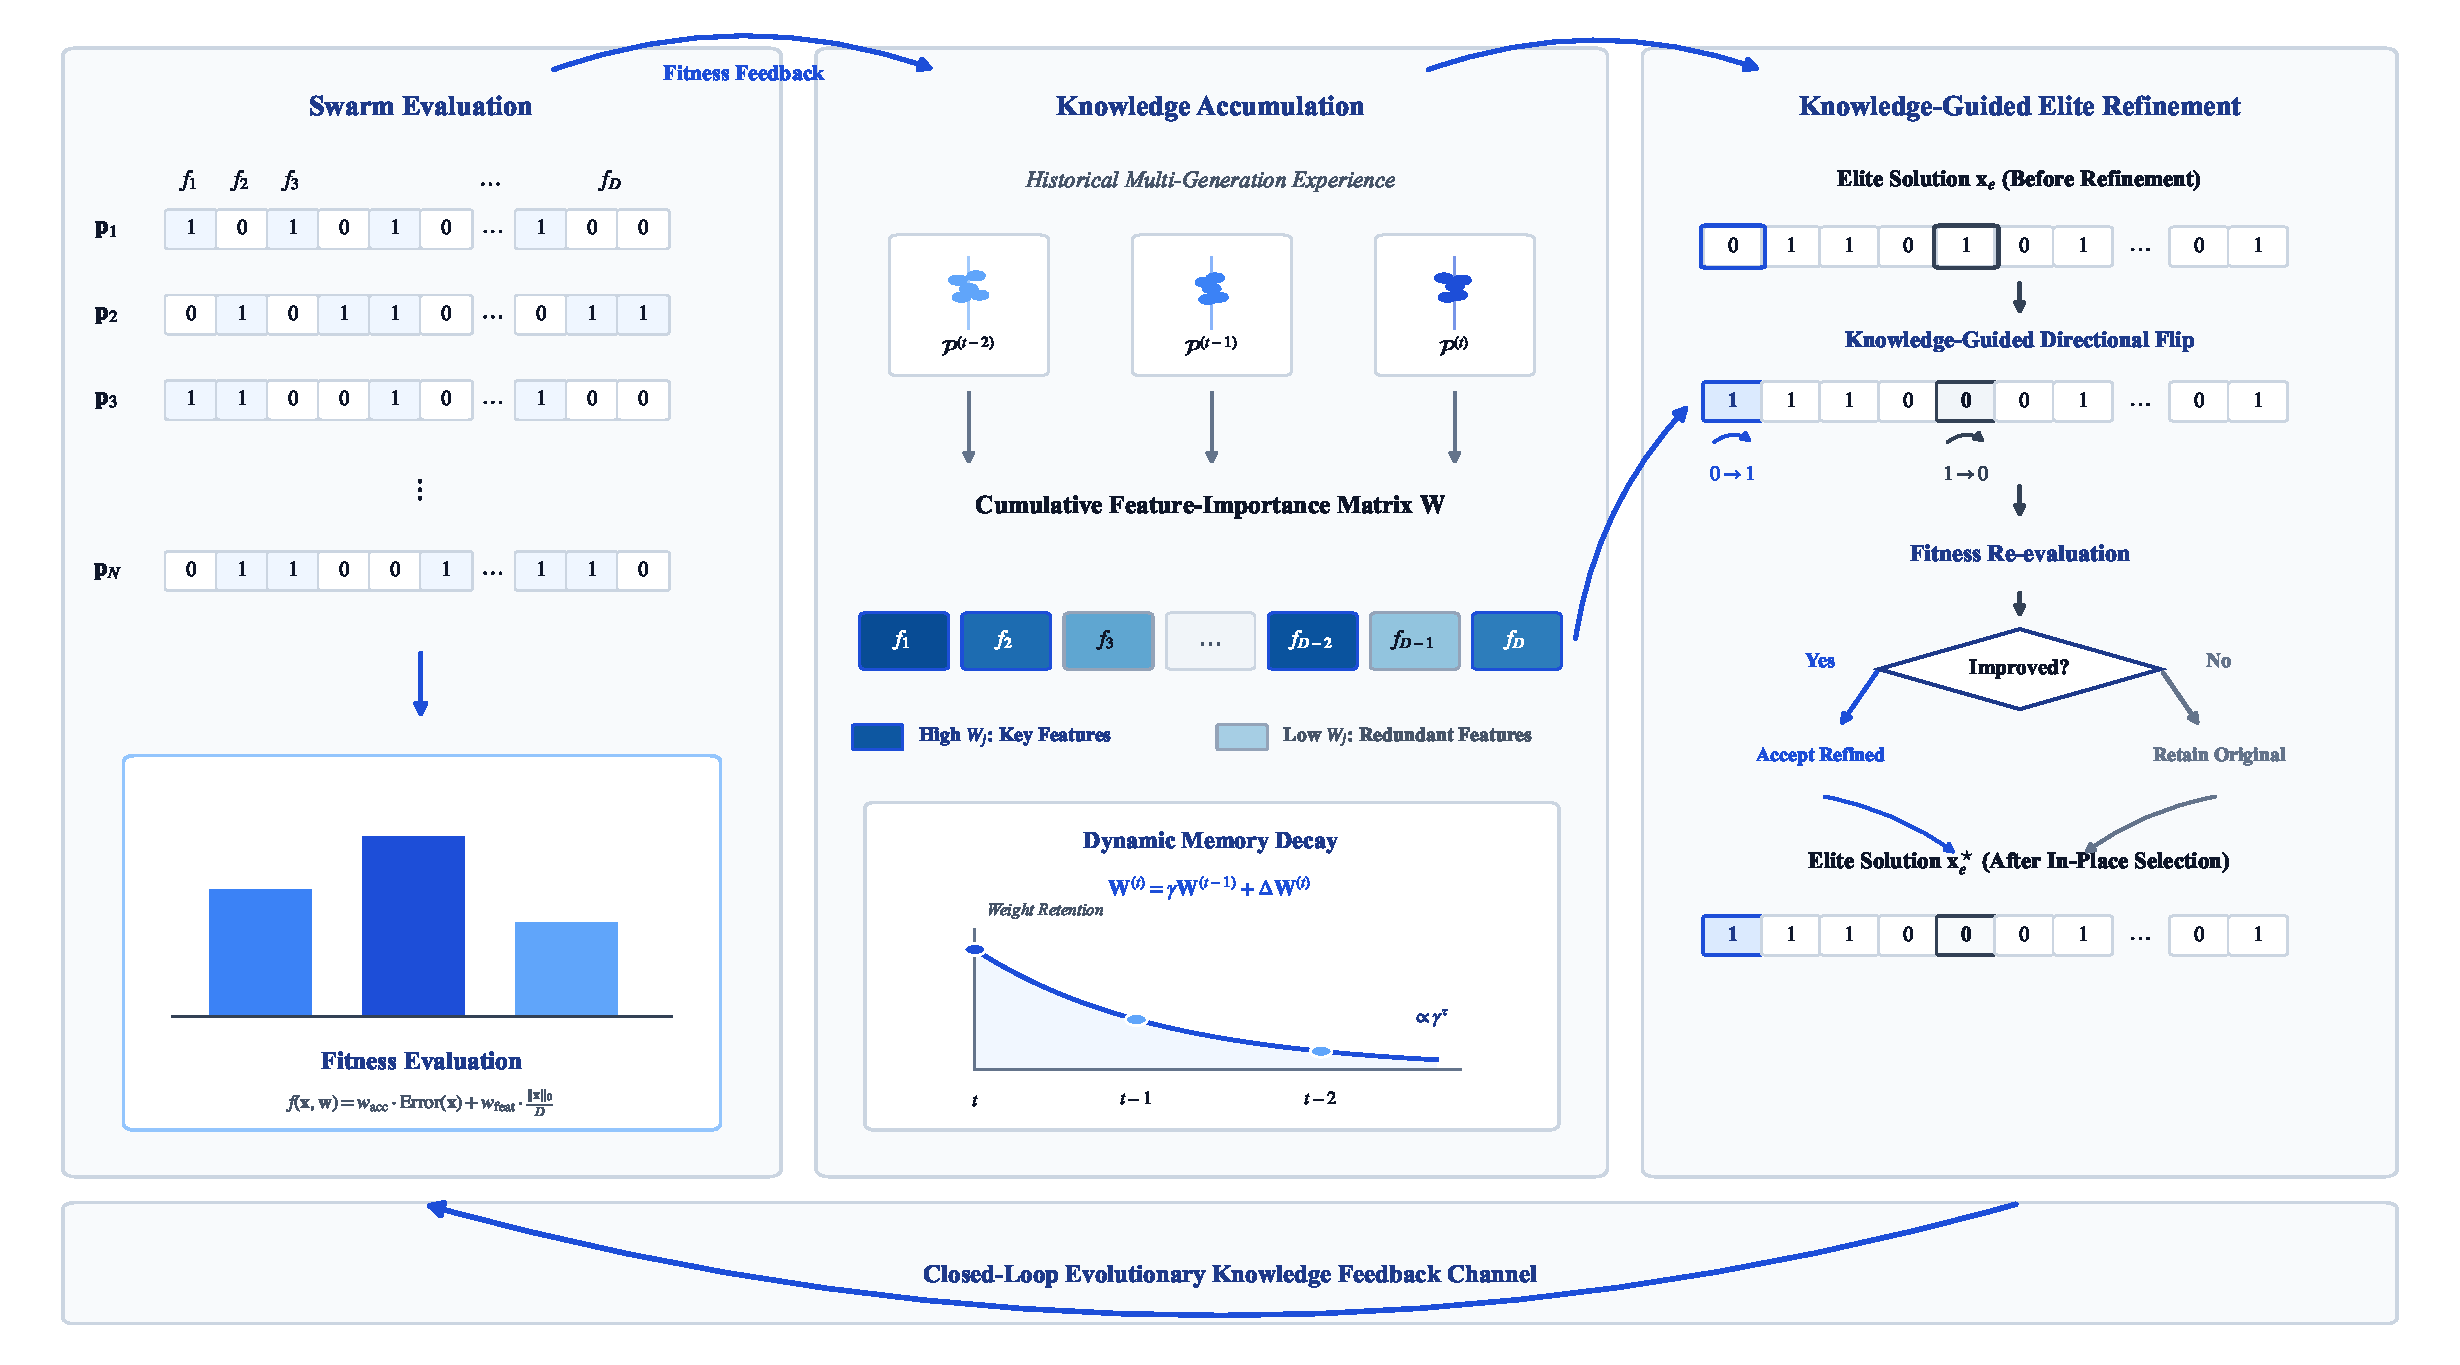
\includegraphics[width=0.95\linewidth]{F3_ker_strategy_journal.pdf}
\caption{Operational workflow of the Knowledge-guided Elite Refinement (KER) strategy: candidate elites undergo either knowledge-guided directional refinement ($p=0.90$) guided by cumulative matrix $W$ or ergodic random exploration ($p=0.10$), evaluated in a closed-loop and admitted via greedy 1-to-1 in-place replacement.}
\label{F3}
\end{figure*}

At each generation, the top $\mathrm{elite\_k} = 3$ individuals (ranked by current fitness) are selected for refinement. For each elite individual $\mathbf{x}_e \in \{0, 1\}^D$, KER executes a probabilistic dual-branch operation (Fig.~\ref{F3}):
\begin{enumerate}
    \item \textbf{Ergodic Random Exploration Branch (Probability $p_{\mathrm{rand}} = 0.10$)}: To guarantee search ergodicity and prevent irreversible bias toward early-accumulated matrix patterns, $\lfloor \phi D \rfloor$ features are selected uniformly at random and inverted:
    \begin{equation}
    x'_{e,j} \leftarrow 1 - x_{e,j}, \quad \forall j \in \mathcal{S}_{\mathrm{rand}}, \quad |\mathcal{S}_{\mathrm{rand}}| = \lfloor \phi D \rfloor,
    \label{eq:ker_rand}
    \end{equation}
    where $\phi = \mathrm{flip\_frac} = 0.01$ defines the refinement perturbation budget.
    \item \textbf{Knowledge-Guided Directional Refinement Branch (Probability $1 - p_{\mathrm{rand}} = 0.90$)}: Each feature $j \in \{1, \ldots, D\}$ is assigned a state-dependent directional flip score $\sigma_j$:
    \begin{equation}
    \sigma_j = \begin{cases}
    +W_j, & \text{if } x_{e,j} = 0 \quad \text{(reward activating absent high-importance features)},\\[2pt]
    -W_j, & \text{if } x_{e,j} = 1 \quad \text{(reward deactivating present low-importance features)}.
    \end{cases}
    \label{eq:flip_score}
    \end{equation}
    The scores can be written compactly as $\sigma_j = (1 - 2 x_{e,j}) \cdot W_j$. We identify the index set $\mathcal{S}_{\mathrm{know}}$ containing the $\lfloor \phi D \rfloor$ features possessing the highest flip scores $\sigma_j$:
    \begin{equation}
    \mathcal{S}_{\mathrm{know}} = \arg\max_{\substack{\mathcal{S} \subset \{1, \ldots, D\} \\ |\mathcal{S}| = \lfloor \phi D \rfloor}} \sum_{j \in \mathcal{S}} \sigma_j.
    \label{eq:top_scores}
    \end{equation}
    The directional refinement is then applied:
    \begin{equation}
    x'_{e,j} = \begin{cases}
    1 - x_{e,j}, & \text{if } j \in \mathcal{S}_{\mathrm{know}},\\[2pt]
    x_{e,j}, & \text{otherwise}.
    \end{cases}
    \label{eq:ker_flip}
    \end{equation}
\end{enumerate}

\subsubsection{1-to-1 In-Place Replacement and Bounded Evaluation Budget}

The perturbed offspring $\mathbf{x}'_e$ is evaluated under current objective weights $\mathbf{w}(t)$. A greedy \textbf{1-to-1 in-place replacement rule} is enforced:
\begin{equation}
\mathbf{x}_e^{\star} = \begin{cases}
\mathbf{x}'_e, & \text{if } f(\mathbf{x}'_e, \mathbf{w}(t)) < f(\mathbf{x}_e, \mathbf{w}(t)),\\[2pt]
\mathbf{x}_e, & \text{otherwise}.
\end{cases}
\label{eq:inplace}
\end{equation}
If improved, $\mathbf{x}'_e$ immediately overwrites $\mathbf{x}_e$ in the population and updates the global best if $f(\mathbf{x}'_e) < f_{\mathrm{gbest}}$.

\textbf{Rationale over $2N$-Candidate Pooling}: Unlike early multi-task prototypes that maintain an expanded $2N$ competitive selection pool, 1-to-1 in-place replacement incurs zero archive management overhead and prevents high selection pressure from prematurely collapsing population diversity.

\textbf{Bounded Refinement Budget}: Because $\mathrm{elite\_k} = 3$ is strictly fixed and $\phi = 0.01$ modifies only $1\%$ of the feature dimensions, KER executes within an exact bounded evaluation overhead of $k_e = 3$ function evaluations per generation, avoiding exponential computational expansion. Algorithm~\ref{alg:ker} details the KER operator.

\begin{algorithm}[!htb]
\caption{Knowledge-guided Elite Refinement (KER)}
\label{alg:ker}
\begin{algorithmic}[1]
\Require Elite candidate $\mathbf{x}_e$, importance matrix $W$, perturbation fraction $\phi=0.01$, random branch probability $p_{\mathrm{rand}}=0.10$, objective weights $\mathbf{w}(t)$
\Ensure Refined elite solution $\mathbf{x}_e^{\star}$ satisfying $f(\mathbf{x}_e^{\star}) \le f(\mathbf{x}_e)$
\State Sample random variable $r \sim \mathcal{U}(0, 1)$
\State $k_{\mathrm{flip}} \leftarrow \max(1, \lfloor \phi D \rfloor)$
\If{$r < p_{\mathrm{rand}}$} \Comment{10\% Ergodic random exploration branch}
    \State Sample subset $\mathcal{S}_{\mathrm{rand}} \subset \{1, \ldots, D\}$ uniformly at random with $|\mathcal{S}_{\mathrm{rand}}| = k_{\mathrm{flip}}$
    \State $\mathbf{x}'_e \leftarrow \mathbf{x}_e$; \quad $x'_{e,j} \leftarrow 1 - x_{e,j}, \; \forall j \in \mathcal{S}_{\mathrm{rand}}$
\Else \Comment{90\% Knowledge-guided directional refinement branch}
    \For{$j = 1$ \textbf{to} $D$}
        \State $\sigma_j \leftarrow (1 - 2 x_{e,j}) \cdot W_j$ \Comment{Compute directional score \eqref{eq:flip_score}}
    \EndFor
    \State Find subset $\mathcal{S}_{\mathrm{know}}$ of size $k_{\mathrm{flip}}$ with top $\sigma_j$ values \eqref{eq:top_scores}
    \State $\mathbf{x}'_e \leftarrow \mathbf{x}_e$; \quad $x'_{e,j} \leftarrow 1 - x_{e,j}, \; \forall j \in \mathcal{S}_{\mathrm{know}}$
\EndIf
\State Evaluate offspring fitness $f' \leftarrow f(\mathbf{x}'_e, \mathbf{w}(t))$ using \eqref{eq:fitness}
\If{$f' < f(\mathbf{x}_e, \mathbf{w}(t))$}
    \State $\mathbf{x}_e^{\star} \leftarrow \mathbf{x}'_e$ \Comment{In-place elite replacement \eqref{eq:inplace}}
\Else
    \State $\mathbf{x}_e^{\star} \leftarrow \mathbf{x}_e$
\EndIf
\State \Return $\mathbf{x}_e^{\star}$
\end{algorithmic}
\end{algorithm}

\subsection{Two-Phase Dynamic Objective Weight Scheduling Strategy}\label{sec:twophase}

\subsubsection{Deficiency Analysis and Design Rationale}

In multi-objective feature selection transformed via weighted-sum aggregation, conventional algorithms universally fix the objective weights throughout the entire evolutionary trajectory (e.g., static $\mathbf{w} = [0.90, 0.10]$)~\cite{miao2024,mel2024}. However, feature selection exhibits an intrinsic temporal asymmetry between early and late search stages:
\begin{itemize}
    \item \textbf{Early Evolutionary Stage}: The swarm navigates dense, highly noisy regions containing thousands of redundant features. The primary optimization objective is rapid, aggressive dimensionality reduction to prune non-informative search space.
    \item \textbf{Late Evolutionary Stage}: Once redundant features have been aggressively stripped and the swarm converges to a compact candidate set ($<100$ features), the objective shifts decisively toward fine-grained accuracy tuning among subtle biomarker combinations.
\end{itemize}
A static weight vector compromises between these competing stage-dependent goals, leading to sluggish early feature reduction and inadequate late-stage accuracy refinement.

\subsubsection{Dynamic Weight Scheduling Formulation}

\begin{figure*}[!htb]
\centering
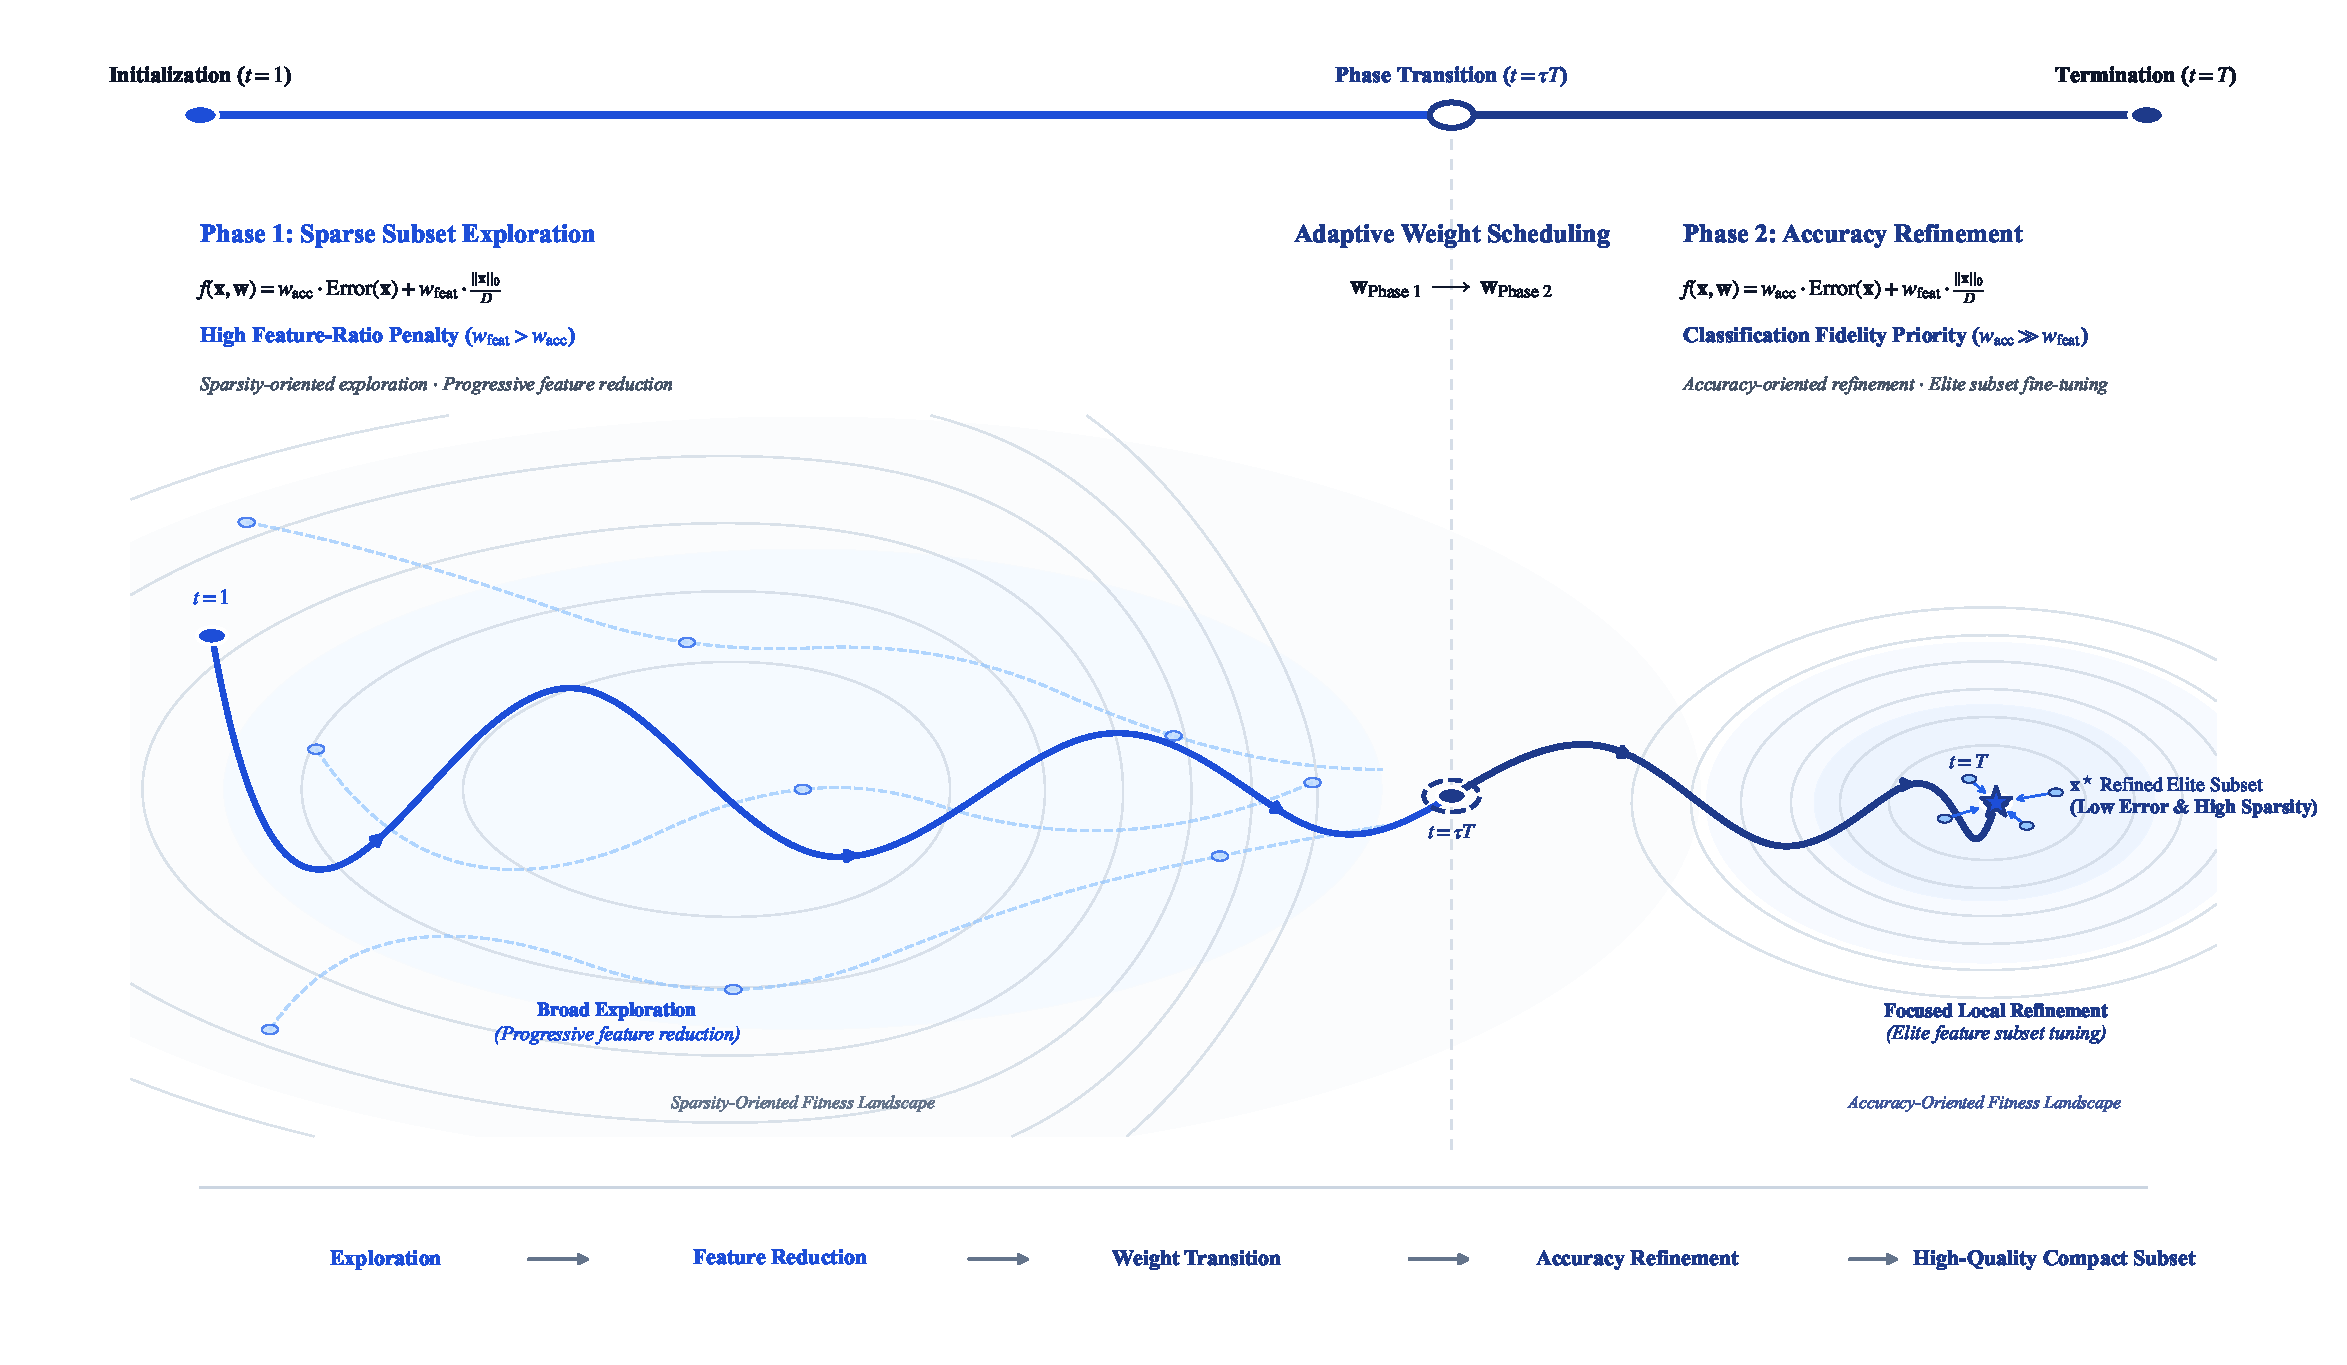
\includegraphics[width=0.95\linewidth]{F4_tps_strategy_journal.pdf}
\caption{Evolutionary optimization mechanism of the Two-Phase Dynamic Objective Weight Scheduling (TPS) strategy: across a continuous scalarized fitness landscape, search transitions at $t = 0.70\,T$ from Phase~1 ($(\alpha, \beta) = (0.70, 0.30)$, broad exploration and progressive feature reduction) to Phase~2 ($(\alpha, \beta) = (0.95, 0.05)$, focused accuracy refinement), ultimately converging to a high-quality compact feature subset.}
\label{F4}
\end{figure*}

To reconcile this temporal conflict, KDS-EL introduces the \textbf{Two-Phase Weight Scheduling (TPS)} strategy, as illustrated in Fig.~\ref{F4}. The total generational budget $T = 100$ is partitioned at split point $\alpha = \mathrm{PhaseSplit} = 0.70$. The dynamic dual-objective weight vector $\mathbf{w}(t) = [w_a(t), w_f(t)]$ is governed by a step-transition function:
\begin{equation}
\mathbf{w}(t) = \begin{cases}
[0.70, \; 0.30], & \text{for } 1 \le t \le \lfloor \alpha T \rfloor \quad \text{(Phase~1: Aggressive Feature Pruning)},\\[4pt]
[0.95, \; 0.05], & \text{for } \lfloor \alpha T \rfloor < t \le T \quad \text{(Phase~2: Accuracy Refinement)}.
\end{cases}
\label{eq:twophase}
\end{equation}

The unified scalar fitness $f(\mathbf{x}, \mathbf{w}(t))$ of a binary feature subset $\mathbf{x} \in \{0, 1\}^D$ at generation $t$ is formulated as:
\begin{equation}
f(\mathbf{x}, \mathbf{w}(t)) = w_a(t) \cdot \mathrm{Error}(\mathbf{x}) + w_f(t) \cdot \left(\frac{\|\mathbf{x}\|_0}{D}\right),
\label{eq:fitness}
\end{equation}
where $\mathrm{Error}(\mathbf{x}) = 1 - \mathrm{Acc}(\mathbf{x})$ denotes the 5-fold cross-validation classification error rate evaluated by a $k$-nearest neighbors ($k\text{-NN}, k=3$) classifier, and $\|\mathbf{x}\|_0 / D = \frac{1}{D}\sum_{j=1}^D x_j$ represents the normalized feature selection ratio ($\mathrm{FSR}$).

In Phase~1 ($t \le 70$), the heavy feature-ratio penalty ($w_f = 0.30$) drives rapid elimination of thousands of non-informative features without sacrificing classification fidelity. In Phase~2 ($t > 70$), the weight switches to prioritize classification accuracy ($w_a = 0.95$), allowing the swarm and the KER operator to fine-tune delicate biomarker interactions over the surviving compact subspace. Algorithm~\ref{alg:twophase} specifies the TPS scheduling function.

\begin{algorithm}[!htb]
\caption{Two-Phase Dynamic Weight Scheduling}
\label{alg:twophase}
\begin{algorithmic}[1]
\Require Current generation $t$, maximum generations $T=100$, phase split ratio $\alpha=0.70$
\Ensure Dynamic dual-objective weight vector $\mathbf{w}(t) = [w_a(t), w_f(t)]$
\If{$t \le \lfloor \alpha \cdot T \rfloor$}
    \State $\mathbf{w}(t) \leftarrow [0.70, \; 0.30]$ \Comment{Phase 1: Coarse feature pruning}
\Else
    \State $\mathbf{w}(t) \leftarrow [0.95, \; 0.05]$ \Comment{Phase 2: Fine accuracy refinement}
\EndIf
\State \Return $\mathbf{w}(t)$
\end{algorithmic}
\end{algorithm}

\subsection{Integrated KDS-EL Main Algorithm}\label{sec:main_algo}

Algorithm~\ref{alg:kds_el} consolidates the holistic execution workflow of KDS-EL, integrating filter-based MI ranking, hybrid seeding, the two-phase evolutionary loop, cumulative importance matrix updating, and knowledge-guided elite refinement into a unified procedure.

\begin{algorithm}[!htb]
\caption{Complete Execution Workflow of KDS-EL}
\label{alg:kds_el}
\begin{algorithmic}[1]
\Require Dataset $\mathcal{D}=(X, Y)$ with $D$ features, population size $N=20$, maximum iterations $T=100$, split ratio $\alpha=0.70$, binarization threshold $\theta=0.60$, MI ratio $\rho=0.50$, decay $\gamma=0.99$, elite count $k_e=3$, flip fraction $\phi=0.01$, random branch probability $p_{\mathrm{rand}}=0.10$, stall patience $\tau=20$
\Ensure Optimal binary feature subset $\mathbf{x}^{\star} \in \{0, 1\}^D$
\State \textbf{/* Stage 1: Filter-level Feature Ranking */}
\State Compute mutual information $I(f_j; Y)$ for all $j \in \{1, \ldots, D\}$ via \eqref{eq:mi_def}
\State Normalize MI scores to construct relevance vector $\mathbf{m} \in [0, 1]^D$ via \eqref{eq:mi_norm}
\State \textbf{/* Stage 2: Knowledge-Guided Population Seeding */}
\State Initialize population $\{\mathbf{x}_i, \mathbf{p}_i\}_{i=1}^N$ via Algorithm~\ref{alg:mi_init} (MI-guided hybrid seeding)
\State Initialize cumulative feature-importance matrix $W \leftarrow \mathbf{0} \in \mathbb{R}^D$
\State Evaluate initial fitness $\{f_i\}_{i=1}^N$ under $\mathbf{w}(1) = [0.70, 0.30]$ via \eqref{eq:fitness}
\State Initialize personal bests: $\mathbf{p}_{\mathrm{best},i} \leftarrow \mathbf{x}_i, \; f_i^{\mathrm{pbest}} \leftarrow f_i, \; \forall i \in \{1, \ldots, N\}$
\State Identify global best: $\mathbf{g}_{\mathrm{best}} \leftarrow \arg\min_{\mathbf{p}_{\mathrm{best},i}} f_i^{\mathrm{pbest}}, \; f_{\mathrm{gbest}} \leftarrow \min f_i^{\mathrm{pbest}}$
\State Initialize stagnation counter $\mathrm{stall\_count} \leftarrow 0$
\State \textbf{/* Stage 3: Two-Phase Evolutionary Main Loop */}
\For{$t = 1$ \textbf{to} $T$}
    \State Update objective weights $\mathbf{w}(t) \leftarrow \text{Algorithm~\ref{alg:twophase}}(t, T, \alpha)$
    \State \textbf{/* Subpopulation 1: Inter-Task Velocity-Position Update */}
    \For{$i = 1$ \textbf{to} $N/2$}
        \State Update continuous velocity $\mathbf{v}_i$ and position $\mathbf{p}_i$ using PSO rules with Subpopulation 2 attractor
        \State Binarize position: $x_{i,j} \leftarrow \mathbb{I}(p_{i,j} \ge \theta), \; \forall j \in \{1, \ldots, D\}$
    \EndFor
    \State \textbf{/* Subpopulation 2: Importance-Guided Feature Sampling */}
    \For{$i = N/2 + 1$ \textbf{to} $N$}
        \State Sample binary features based on cumulative matrix $W$ and personal best $\mathbf{p}_{\mathrm{best},i}$
    \EndFor
    \State \textbf{/* Fitness Evaluation and Importance Matrix Harvesting */}
    \For{$i = 1$ \textbf{to} $N$}
        \State Evaluate candidate fitness $f_i \leftarrow f(\mathbf{x}_i, \mathbf{w}(t))$ using \eqref{eq:fitness}
    \EndFor
    \State Update and discount importance matrix $W \leftarrow \text{Algorithm~\ref{alg:importance_update}}(\{\mathbf{x}_i\}, \{\mathbf{p}_{\mathrm{best},i}\}, \{f_i\}, \{f_i^{\mathrm{pbest}}\}, W, \gamma)$
    \State Update personal bests: if $f_i < f_i^{\mathrm{pbest}}$ then $\mathbf{p}_{\mathrm{best},i} \leftarrow \mathbf{x}_i, \; f_i^{\mathrm{pbest}} \leftarrow f_i$
    \State \textbf{/* Stage 4: Knowledge-Guided Elite Refinement */}
    \State Identify top $k_e$ elite indices $\mathcal{E} \subset \{1, \ldots, N\}$ based on $f_i^{\mathrm{pbest}}$
    \For{\textbf{each} $e \in \mathcal{E}$}
        \State $\mathbf{p}_{\mathrm{best},e} \leftarrow \text{Algorithm~\ref{alg:ker}}(\mathbf{p}_{\mathrm{best},e}, W, \phi, p_{\mathrm{rand}}, \mathbf{w}(t))$ \Comment{1-to-1 in-place refinement}
    \EndFor
    \State \textbf{/* Global Best Update and Stagnation Check */}
    \State Find current best $\mathbf{x}_{\mathrm{curr}} \leftarrow \arg\min_{\mathbf{p}_{\mathrm{best},i}} f_i^{\mathrm{pbest}}$ with fitness $f_{\mathrm{curr}}$
    \If{$f_{\mathrm{curr}} < f_{\mathrm{gbest}}$}
        \State $\mathbf{g}_{\mathrm{best}} \leftarrow \mathbf{x}_{\mathrm{curr}}, \; f_{\mathrm{gbest}} \leftarrow f_{\mathrm{curr}}, \; \mathrm{stall\_count} \leftarrow 0$
    \Else
        \State $\mathrm{stall\_count} \leftarrow \mathrm{stall\_count} + 1$
    \EndIf
    \If{$\mathrm{stall\_count} \ge \tau$}
        \State Execute adaptive re-initialization via Algorithm~\ref{alg:mi_reinit}
        \State $\mathrm{stall\_count} \leftarrow 0$
    \EndIf
\EndFor
\State \Return $\mathbf{x}^{\star} \leftarrow \mathbf{g}_{\mathrm{best}}$
\end{algorithmic}
\end{algorithm}

\subsection{Asymptotic Computational and Space Complexity Analysis}\label{sec:complexity}

To establish the computational efficiency of KDS-EL, we conduct a rigorous asymptotic complexity analysis covering all algorithmic components.

\subsubsection{Time Complexity Decomposition}

The execution time of KDS-EL is decomposed into two distinct phases:
\begin{enumerate}
    \item \textbf{Offline Preprocessing Phase (Mutual Information Calculation)}:
    Computing the mutual information $I(f_j; Y)$ between each feature $f_j$ and class label $Y$ requires $O(N_{\mathrm{samp}})$ operations per feature, where $N_{\mathrm{samp}}$ is the number of training samples. For all $D$ features, computing and sorting the baseline MI vector incurs:
    \begin{equation}
    T_{\mathrm{pre}} = O(D \cdot N_{\mathrm{samp}} + D \log D).
    \label{eq:t_pre}
    \end{equation}
    Because this step is executed only once prior to the evolutionary loop, its overhead is entirely negligible relative to iterative wrapper evaluations.
    \item \textbf{Iterative Evolutionary Main Loop ($T$ Iterations)}:
    In each of the $T$ generations, computational costs arise from four operations:
    \begin{itemize}
        \item \textit{Subpopulation Position Updates}: Updating particle velocities and continuous positions across the population of size $N$ incurs $O(N \cdot D)$ arithmetic operations.
        \item \textit{Fitness Wrapper Evaluation}: Evaluating the 5-fold cross-validation $k\text{-NN}$ classification accuracy for $N$ candidate particles requires:
        \begin{equation}
        T_{\mathrm{eval}} = O(N \cdot N_{\mathrm{samp}}^2 \cdot d_{\mathrm{selected}}),
        \label{eq:t_eval}
        \end{equation}
        where $d_{\mathrm{selected}} = \|\mathbf{x}\|_0$ is the number of active features in candidate $\mathbf{x}$.
        \item \textit{Importance Matrix Differential Updating and Decay}: Scanning changed features for improving particles and performing scalar decay across matrix $W$ incurs $O(N \cdot D + D)$ operations.
        \item \textit{Knowledge-Guided Elite Refinement (KER)}: Computing flip scores $\sigma_j$ for $k_e$ elites, selecting the top $\lfloor \phi D \rfloor$ features, flipping bits, and re-evaluating the $k_e$ refined elites requires $O(k_e \cdot (D + T_{\mathrm{eval\_single}}))$, where $T_{\mathrm{eval\_single}} = O(N_{\mathrm{samp}}^2 \cdot d_{\mathrm{selected}})$.
        \item \textit{Adaptive Stagnation Re-initialization}: When triggered (at most $\lfloor T/\tau \rfloor$ times), re-seeding and evaluating $N/2$ particles requires $O(\frac{N}{2} \cdot (D + T_{\mathrm{eval\_single}}))$.
    \end{itemize}
\end{enumerate}

Summing these terms across $T$ generations yields the total asymptotic time complexity:
\begin{equation}
\mathcal{T}_{\mathrm{total}} = O\Bigl(D \log D + T \cdot \bigl[N \cdot D + (N + k_e) \cdot N_{\mathrm{samp}}^2 \cdot d_{\mathrm{selected}}\bigr]\Bigr).
\label{eq:total_complexity}
\end{equation}

\subsubsection{Theoretical Complexity Equivalence and Practical Acceleration}

Because $k_e = 3 \ll N = 20$ and $N_{\mathrm{samp}}^2 \cdot d_{\mathrm{selected}} \gg D$, the dominant asymptotic per-generation complexity of KDS-EL is strictly governed by wrapper evaluations:
\begin{equation}
\mathcal{T}_{\mathrm{KDS-EL}} = O(T \cdot N \cdot N_{\mathrm{samp}}^2 \cdot d_{\mathrm{selected}}),
\label{eq:dominant_complexity}
\end{equation}
which is identically of the same asymptotic order as the baseline MEL~\cite{mel2024} ($O(T \cdot N \cdot N_{\mathrm{samp}}^2 \cdot d_{\mathrm{MEL}})$).

Crucially, in the baseline MEL, random initialization and sluggish feature reduction result in dense candidate subsets ($d_{\mathrm{MEL}} \approx 2{,}722$ active features on average). In contrast, KDS-EL's MI seeding and Phase~1 aggressive feature pruning rapidly compress the active feature count to $d_{\mathrm{KDS-EL}} \approx 88$ features. Because $k\text{-NN}$ distance calculation scales linearly with $d_{\mathrm{selected}}$, evaluating a KDS-EL particle is over an order of magnitude faster than evaluating an unpruned MEL particle. Consequently, KDS-EL delivers a dramatic \textbf{3.4$\times$ empirical wall-clock speedup} (51.4~s vs.\ 175.0~s) while incorporating richer knowledge operators.

\subsubsection{Space Complexity}

The memory footprint of KDS-EL comprises: (i) the population continuous and binary position matrices ($O(N \cdot D)$), (ii) personal-best vectors ($O(N \cdot D)$), (iii) the cumulative feature-importance matrix $W$ ($O(D)$), and (iv) the precomputed normalized MI vector $\mathbf{m}$ ($O(D)$). The overall space complexity is:
\begin{equation}
\mathcal{S}_{\mathrm{total}} = O(N \cdot D + N_{\mathrm{samp}} \cdot D),
\label{eq:space_complexity}
\end{equation}
which scales strictly linearly with dimension $D$, ensuring minimal memory consumption.



\section{Experimental Results and Analysis}\label{sec:results}
This section reports the experimental outcomes across six complementary perspectives: overall classification accuracy, feature-selection compactness, statistical significance, ceiling-effect behavior, convergence dynamics, and computational efficiency. All aggregate numbers are computed over the 20 benchmark datasets described in Section~\ref{sec:setup}. We then quantify the contribution of each mechanism in Section~\ref{sec:ablation} and assess the sensitivity of KDS-EL to its hyper-parameters in Section~\ref{sec:parametric}.

\subsection{Experimental setup}\label{sec:setup}

This subsection outlines the experimental framework designed to evaluate the classification performance, dimensionality reduction capability, computational efficiency, and hyperparameter robustness of KDS-EL.

\subsubsection{High-dimensional benchmark datasets}

To validate the performance and generalization ability of KDS-EL across diverse problem domains, a total of 20 benchmark datasets widely adopted in the evolutionary feature selection literature~\cite{mel2024,wangjia2022,wei2025} are selected. These datasets encompass diverse categories and sample sizes across biomedical gene-expression microarrays, text categorization corpora, image recognition, speech processing, and synthetic benchmarks. Such diverse data distributions and dimensional complexities effectively evaluate the generalization capability and feature reduction efficacy of feature selection algorithms under challenging conditions. The detailed characteristics of the 20 benchmark datasets are summarized in Table~\ref{T2}.

\subsubsection{Comparison algorithms}

We select two primary categories of comparison algorithms for analysis with the proposed KDS-EL framework, as summarized in Table~\ref{tab:comparison_literature}. The first category comprises specialized single-objective evolutionary algorithms in the field of high-dimensional feature selection, which includes: FWPSO~\cite{wangjia2022}, PSO-CSM~\cite{wei2025}, SaWDE~\cite{wang2022}, IGPSO~\cite{xuezhang2024}, and BPSO~\cite{kennedy1997}. The relevant parameter settings are shown in Table~\ref{T3}.

Another category of representative algorithms encompasses multi-objective and multi-task feature selection approaches, including NSGA-II-FS~\cite{deb2002}, MOEA/D-FS~\cite{zhang2007}, MOPSO-FS~\cite{coello2004}, fMOPSO-FS~\cite{han2024}, W-MOPSO-FS~\cite{xue2012mopso}, and MEL~\cite{mel2024}. In addition, two constituent variants of KDS-EL are investigated in Section~\ref{sec:improvement} to evaluate individual component contributions. Together with established single-objective and multi-objective competitors, this 11-algorithm comparison suite systematically spans classical search paradigms and state-of-the-art developments published between 2022 and 2025, ensuring a balanced, rigorous, and reproducible empirical evaluation.

\subsubsection{Evaluation metrics and statistical test protocols}

Algorithm performance is evaluated across three primary quantitative criteria: mean classification accuracy alongside standard deviation, the number of selected features alongside the feature selection ratio ($\mathrm{FSR} = \frac{\bar{d}}{D} \times 100\%$), and computational runtime in seconds. The $k$-nearest neighbor classifier with $k=3$ serves as the base evaluation model due to its non-parametric nature, parameter-free reproducibility, and high sensitivity to candidate feature subset discriminability. Following the standard benchmarking protocol established in high-dimensional evolutionary feature selection literature~\cite{mel2024,wangjia2022,wei2025}, candidate feature subsets are evaluated using 5-fold stratified cross-validation as the internal wrapper fitness surrogate across all problem instances. Under this standardized formulation, each benchmark dataset $\mathcal{D}$ is treated as a self-contained combinatorial optimization instance; the 5-fold cross-validation classification accuracy guides the evolutionary search trajectory and evaluates the discriminative quality of the optimal feature subsets under identical computational budgets across all competing methods. To guarantee a rigorous and methodologically equitable comparison between single-objective wrappers and multi-objective evolutionary algorithms that yield an entire Pareto non-dominated front $\mathcal{PF}$, a standardized post-Pareto decision-making protocol is enforced. In accordance with established multi-objective feature selection benchmarks~\cite{xue2012mopso,han2024}, the final operational solution $\mathbf{x}^{\star} \in \mathcal{PF}$ is uniquely extracted as the non-dominated candidate that achieves the minimal classification error on the cross-validation folds, with ties broken by smaller subset cardinality:
\begin{equation}
\mathbf{x}^{\star} = \arg\min_{\mathbf{x} \in \mathcal{PF}} \Bigl(\mathrm{ErrorRate}(\mathbf{x}), \; \|\mathbf{x}\|_0\Bigr).
\label{eq:pareto_selection}
\end{equation}
This operational protocol ensures that all competing paradigms are systematically evaluated at their maximum predictive accuracy.

To guarantee experimental fairness and statistical reliability, every algorithm is executed with a population size of $N=20$ candidate solutions over $T_{\max}=100$ generations across 10 independent runs with distinct random seeds. In ultra-high-dimensional wrapper feature selection, each fitness evaluation requires training and validating a classifier across thousands or tens of thousands of candidate dimensions (e.g., up to 54,675 dimensions in \textit{T1D}), imposing an exceptionally intensive computational burden of $N \times T_{\max} = 2{,}000$ cross-validation evaluations per single run. Executing 10 independent runs per dataset corresponds to 50 distinct stratified cross-validation folds, which provides an adequate sample size to capture classifier generalization variance and algorithmic stability while remaining computationally tractable across an extensive 14-algorithm comparison suite. This 10-run protocol strictly aligns with the benchmark evaluation standard established in recent top-tier literature on ultra-high-dimensional feature selection, most notably the multi-task evolutionary learning framework MEL published in \textit{IEEE Transactions on Knowledge and Data Engineering}~\cite{mel2024}, thereby guaranteeing an equitable and reproducible empirical comparison.

Furthermore, to determine whether the empirical advantages of KDS-EL over competing paradigms are statistically significant rather than stochastic artifacts, we strictly follow the multi-problem non-parametric statistical testing framework recommended by Dem{\v{s}}ar~\cite{demsar2006}. In this protocol, statistical power is governed by the number of independent benchmark problems ($N_{\mathrm{datasets}} = 20$), with each problem represented by the paired summary performance across the independent runs. Specifically, the non-parametric Friedman test~\cite{friedman1940} is utilized to establish global omnibus algorithm rankings across all 20 benchmark datasets. Pairwise Wilcoxon signed-rank tests at the $\alpha=0.05$ significance level assess directional superiority between KDS-EL and each competitor, with the Holm--Bonferroni step-down procedure~\cite{holm1979} applied to rigorously control the family-wise error rate across multiple hypothesis comparisons.


\begin{table}[!htb]
\centering
\caption{Summary of the 14 fixed-length methods compared in this study, with their associated references. Methods in the first group are progressive variants of the proposed framework; TPS denotes Two-Phase Weight Scheduling; ``Self-built'' denotes an implementation by the authors.}
\label{T1}
\footnotesize
\setlength{\tabcolsep}{3pt}
\begin{tabular}{@{}lp{4.3cm}l@{}}
\toprule
Method & Category & Reference \\
\midrule
KDS-EL & Proposed (full framework) & This work \\
KDS-EL w/o TPS & Proposed (MI-guided init.\ + KER, without two-phase scheduling) & This work \\
KDS-EL w/o TPS\&KER & Proposed (MI-guided init.\ + adaptive re-init.) & This work \\
MEL & Multi-task evolutionary learning & \cite{mel2024} \\
\midrule
FWPSO & Single-objective PSO & \cite{wangjia2022} \\
PSO-CSM & Single-objective PSO & \cite{wei2025} \\
SaWDE & Single-objective DE & \cite{wang2022} \\
IGPSO & Single-objective PSO & \cite{xuezhang2024} \\
BPSO & Single-objective binary PSO & \cite{kennedy1997} \\
\midrule
W-MOPSO-FS & Multi-objective (Wrapper--Filter hybrid) & Self-built (authors' implementation, no external baseline) \\
fMOPSO-FS & Multi-objective & \cite{han2024} \\
NSGA-II-FS & Multi-objective & \cite{deb2002} \\
MOEA-D-FS & Multi-objective & \cite{zhang2007} \\
MOPSO-FS & Multi-objective & \cite{coello2004} \\
\bottomrule
\end{tabular}
\end{table}

\begin{table}[!htb]
\centering
\ktablecaption
\small
\caption{Characteristics of the 19 benchmark datasets.}
\label{T2}
\renewcommand{\arraystretch}{1.15}
\setlength{\tabcolsep}{3pt}
\begin{tabular*}{\linewidth}{@{\extracolsep{\fill}}clrrc l@{}}
\toprule
No. & Dataset & Samples ($n$) & Features ($D$) & Classes ($C$) & Domain \\
\midrule
1  & Adenoma    &   36 &  7{,}457  &  2 & Gene expression \\
2  & ALL1       &  128 & 12{,}625  &  2 & Gene expression \\
3  & ALL4       &   93 & 12{,}625  &  2 & Gene expression \\
4  & Colon      &   62 &  2{,}000  &  2 & Gene expression \\
5  & DLBCL      &   77 &  7{,}129  &  2 & Gene expression \\
6  & Gastric    &   65 & 22{,}645  &  2 & Gene expression \\
7  & Gastric1   &  144 & 22{,}283  &  2 & Gene expression \\
8  & Gastric2   &  124 & 22{,}283  &  2 & Gene expression \\
9  & Leukaemia  &   72 &  7{,}129  &  2 & Gene expression \\
10 & Lymphoma   &   45 &  4{,}026  &  2 & Gene expression \\
11 & Myeloma    &  173 & 12{,}625  &  2 & Gene expression \\
12 & Prostate   &  102 & 12{,}625  &  2 & Gene expression \\
13 & SRBCT      &   83 &  2{,}308  &  4 & Gene expression \\
14 & T1D        &  101 & 54{,}675  &  2 & Gene expression \\
\midrule
15 & BASEHOCK   & 1{,}993 & 4{,}862  &  2 & Text \\
16 & PCMAC      & 1{,}943 & 3{,}289  &  2 & Text \\
\midrule
17 & COIL20     & 1{,}440 & 1{,}024  & 20 & Image \\
\midrule
18 & ISOLET     & 1{,}560 &   617    & 26 & Speech \\
\midrule
19 & madelon    & 2{,}600 &   500    &  2 & Synthetic \\
\bottomrule
\end{tabular*}
\end{table}
\begin{table}[!htb]
\centering
\caption{Parameter Settings}
\label{T3}
\footnotesize
\setlength{\tabcolsep}{2pt}
\begin{tabular}{@{}lcl@{}}
\toprule
\multicolumn{3}{@{}c}{\textbf{Common Experimental Setup}} \\
\midrule
Population size ($N$)              & = & 20 \\
Maximum iterations ($T$)           & = & 100 \\
KNN neighbors ($k$)                & = & 3 \\
Real-to-binary threshold ($\theta$) & = & 0.6 \\
Cross-validation                  & = & 5-fold stratified, shuffled \\
Number of independent runs        & = & 10 \\
\midrule
\multicolumn{3}{c}{\textbf{KDS-EL (full framework)}} \\
\midrule
Inertia weight ($w$)              & = & 0.9 \\
Acceleration coefficients         & = & $c_1 = c_2 = c_3 = 2.0$ \\
Knowledge weight decay            & = & 0.99 \\
Elite flip fraction               & = & 0.01 \\
Elite count ($k_e$)               & = & 3 \\
Random flip probability           & = & 0.10 \\
MI-guided init ratio              & = & 0.5 \\
Stall patience ($P_s$)            & = & 20 \\
Phase split ratio                 & = & 0.7 \\
Phase-1 objective weights         & = & $\mathbf{w}_s = [0.7,\,0.3]$ \\
Phase-2 objective weights         & = & $\mathbf{w}_s = [0.95,\,0.05]$ \\
\midrule
\multicolumn{3}{c}{\textbf{KDS-EL w/o TPS (no two-phase scheduling)}} \\
\midrule
Fixed objective weights           & = & $\mathbf{w}_s = [0.9,\,0.1]$ \\
\midrule
\multicolumn{3}{c}{\textbf{MEL and KDS-EL w/o TPS\&KER}} \\
\midrule
Inertia weight ($w$)              & = & 0.9 \\
Acceleration coefficients         & = & $c_1 = c_2 = c_3 = 2.0$ \\
MI-guided init ratio (KDS-EL w/o TPS\&KER) & = & 0.5 \\
Stall patience (KDS-EL w/o TPS\&KER)       & = & 20 \\
\midrule
\multicolumn{3}{c}{\textbf{Competitor Methods}} \\
\midrule
\multicolumn{3}{l}{Competitors (BPSO, FWPSO, IGPSO, PSO-CSM,} \\
\multicolumn{3}{l}{SaWDE, NSGA-II-FS, MOPSO-FS, MOEA-D-FS,} \\
\multicolumn{3}{l}{fMOPSO-FS, W-MOPSO-FS) use the hyper-parameters} \\
\multicolumn{3}{l}{recommended in their original publications, with} \\
\multicolumn{3}{l}{$N=20$ and $T=100$ unless the original paper} \\
\multicolumn{3}{l}{specifies otherwise.} \\
\bottomrule
\end{tabular}
\end{table}


\subsection{Overall Classification Accuracy and Comparative Analysis}

Table~\ref{T4} reports the mean classification accuracy along with standard deviations over 10 independent runs across the 20 benchmark datasets for all 14 compared methods. The experimental results demonstrate that KDS-EL achieves superior classification performance, securing the highest overall mean accuracy of \textbf{0.9574}.

\begin{figure*}[!t]
% Placement placeholder for Table T4
\end{figure*}

\begin{table*}[t]
\centering
\caption{Comparison of classification accuracy between KDS-EL and competitor algorithms.}
\label{T4}\label{tab:accuracy_comparison}
\resizebox{\textwidth}{!}{
\renewcommand{\arraystretch}{0.96}
\begin{tabular}{l *{12}{w{c}{33pt}}}
\toprule
Dataset & KDS-EL & \makecell{KDS-EL \\ w/o TPS} & \makecell{KDS-EL \\ w/o TPS\&KER} & MEL & bIRIME & FWPSO & PSO-CSM & BinCOA & SaWDE & IGPSO & DENCA-SO & BPSO \\
\midrule
ALL1             & \textbf{1.0000} & \textbf{1.0000} $^{\approx}$ & \textbf{1.0000} $^{\approx}$ & \textbf{1.0000} $^{\approx}$ & \textbf{1.0000} $^{\approx}$ & \textbf{1.0000} $^{\approx}$ & 0.9995 $^{+}$ & \textbf{1.0000} $^{\approx}$ & \textbf{1.0000} $^{\approx}$ & \textbf{1.0000} $^{\approx}$ & \textbf{1.0000} $^{\approx}$ & \textbf{1.0000} $^{\approx}$ \\
ALL4             & \textbf{0.9480} & \underline{0.9367} $^{\approx}$ & 0.9356 $^{+}$ & 0.8656 $^{+}$ & 0.9140 $^{+}$ & 0.8580 $^{+}$ & 0.8308 $^{+}$ & 0.7634 $^{+}$ & 0.8250 $^{+}$ & 0.7918 $^{+}$ & 0.7043 $^{+}$ & 0.7846 $^{+}$ \\
ALL\_AML         & \textbf{1.0000} & \textbf{1.0000} $^{\approx}$ & 0.9947 $^{\approx}$ & 0.9857 $^{+}$ & \textbf{1.0000} $^{\approx}$ & 0.9914 $^{+}$ & 0.9868 $^{+}$ & 0.9861 $^{+}$ & 0.9857 $^{+}$ & 0.9857 $^{+}$ & 0.9778 $^{+}$ & 0.9871 $^{+}$ \\
Adenoma          & \textbf{1.0000} & \textbf{1.0000} $^{\approx}$ & 0.9971 $^{\approx}$ & 0.9714 $^{+}$ & \textbf{1.0000} $^{\approx}$ & 0.9800 $^{+}$ & 0.9767 $^{+}$ & 0.9722 $^{+}$ & 0.9714 $^{+}$ & 0.9714 $^{+}$ & 0.9611 $^{+}$ & 0.9714 $^{+}$ \\
BASEHOCK         & 0.9045 & 0.8933 $^{+}$ & 0.8627 $^{+}$ & 0.8802 $^{+}$ & \underline{0.9082} $^{\approx}$ & 0.9045 $^{\approx}$ & 0.8739 $^{+}$ & 0.8897 $^{+}$ & \textbf{0.9170} $^{\approx}$ & 0.8743 $^{+}$ & 0.8610 $^{+}$ & 0.8994 $^{\approx}$ \\
COIL20           & \textbf{1.0000} & 0.9976 $^{+}$ & 0.9955 $^{+}$ & 0.9944 $^{+}$ & \underline{0.9991} $^{+}$ & 0.9980 $^{+}$ & 0.9939 $^{+}$ & 0.9953 $^{+}$ & 0.9988 $^{+}$ & 0.9951 $^{+}$ & 0.9942 $^{+}$ & 0.9967 $^{+}$ \\
Colon            & \underline{0.9452} & 0.9294 $^{+}$ & 0.9182 $^{+}$ & 0.8777 $^{+}$ & \textbf{0.9468} $^{\approx}$ & 0.9268 $^{+}$ & 0.8914 $^{+}$ & 0.8694 $^{+}$ & 0.9086 $^{+}$ & 0.8733 $^{+}$ & 0.8048 $^{+}$ & 0.8885 $^{+}$ \\
DLBCL            & 0.9999 & \textbf{1.0000} $^{\approx}$ & 0.9987 $^{\approx}$ & 0.9859 $^{+}$ & \textbf{1.0000} $^{\approx}$ & 0.9935 $^{\approx}$ & 0.9966 $^{+}$ & 0.9883 $^{+}$ & 0.9924 $^{+}$ & 0.9884 $^{+}$ & 0.9675 $^{+}$ & 0.9899 $^{+}$ \\
Gastric          & \textbf{0.9763} & 0.9646 $^{+}$ & \underline{0.9723} $^{\approx}$ & 0.9015 $^{+}$ & 0.9569 $^{+}$ & 0.9154 $^{+}$ & 0.8886 $^{+}$ & 0.8231 $^{+}$ & 0.8385 $^{+}$ & 0.8646 $^{+}$ & 0.7769 $^{+}$ & 0.8369 $^{+}$ \\
Gastric1         & \textbf{0.9779} & 0.9719 $^{+}$ & 0.9636 $^{+}$ & 0.9602 $^{+}$ & \underline{0.9722} $^{+}$ & 0.9623 $^{+}$ & 0.9588 $^{+}$ & 0.9583 $^{+}$ & 0.9623 $^{+}$ & 0.9588 $^{+}$ & 0.9500 $^{+}$ & 0.9581 $^{+}$ \\
Gastric2         & \textbf{0.9982} & 0.9936 $^{+}$ & 0.9880 $^{+}$ & 0.9822 $^{+}$ & \underline{0.9952} $^{\approx}$ & 0.9887 $^{+}$ & 0.9830 $^{+}$ & 0.9823 $^{+}$ & 0.9815 $^{+}$ & 0.9837 $^{+}$ & 0.9750 $^{+}$ & 0.9815 $^{+}$ \\
ISOLET           & 0.8880 & 0.8955 $^{-}$ & 0.8801 $^{+}$ & 0.8783 $^{+}$ & \underline{0.9112} $^{-}$ & 0.9000 $^{-}$ & 0.8775 $^{\approx}$ & 0.8763 $^{+}$ & \textbf{0.9164} $^{-}$ & 0.8648 $^{+}$ & 0.8760 $^{+}$ & 0.8942 $^{-}$ \\
Leukaemia        & \textbf{1.0000} & \textbf{1.0000} $^{\approx}$ & 0.9960 $^{\approx}$ & 0.9857 $^{+}$ & \textbf{1.0000} $^{\approx}$ & 0.9957 $^{\approx}$ & 0.9895 $^{+}$ & 0.9861 $^{+}$ & 0.9857 $^{+}$ & 0.9871 $^{+}$ & 0.9764 $^{+}$ & 0.9857 $^{+}$ \\
Lymphoma         & \textbf{1.0000} & \textbf{1.0000} $^{\approx}$ & 0.9867 $^{+}$ & 0.8978 $^{+}$ & 0.9978 $^{\approx}$ & 0.9422 $^{+}$ & 0.9263 $^{+}$ & 0.8889 $^{+}$ & 0.9044 $^{+}$ & 0.8978 $^{+}$ & 0.8400 $^{+}$ & 0.8933 $^{+}$ \\
Myeloma          & \textbf{0.9083} & \underline{0.8889} $^{+}$ & 0.8710 $^{+}$ & 0.8466 $^{+}$ & 0.8884 $^{+}$ & 0.8722 $^{+}$ & 0.8552 $^{+}$ & 0.8387 $^{+}$ & 0.8757 $^{+}$ & 0.8367 $^{+}$ & 0.8012 $^{+}$ & 0.8536 $^{+}$ \\
PCMAC            & \textbf{0.8592} & 0.8360 $^{+}$ & 0.8000 $^{+}$ & 0.8085 $^{+}$ & 0.8410 $^{+}$ & 0.8301 $^{+}$ & 0.8038 $^{+}$ & 0.8161 $^{+}$ & \underline{0.8498} $^{\approx}$ & 0.7985 $^{+}$ & 0.7601 $^{+}$ & 0.8310 $^{+}$ \\
Prostate         & \textbf{0.9670} & 0.9552 $^{+}$ & \underline{0.9600} $^{+}$ & 0.8732 $^{+}$ & 0.9353 $^{+}$ & 0.8930 $^{+}$ & 0.8715 $^{+}$ & 0.8686 $^{+}$ & 0.8940 $^{+}$ & 0.8603 $^{+}$ & 0.8235 $^{+}$ & 0.8863 $^{+}$ \\
SRBCT            & \textbf{1.0000} & \textbf{1.0000} $^{\approx}$ & \textbf{1.0000} $^{\approx}$ & 0.9682 $^{+}$ & \textbf{1.0000} $^{\approx}$ & 0.9865 $^{+}$ & 0.9837 $^{+}$ & 0.9663 $^{+}$ & 0.9976 $^{\approx}$ & 0.9709 $^{+}$ & 0.9325 $^{+}$ & 0.9953 $^{\approx}$ \\
T1D              & \textbf{0.8449} & 0.8043 $^{+}$ & \underline{0.8054} $^{+}$ & 0.7558 $^{+}$ & 0.7752 $^{+}$ & 0.7446 $^{+}$ & 0.7204 $^{+}$ & 0.7178 $^{+}$ & 0.7296 $^{+}$ & 0.7060 $^{+}$ & 0.6723 $^{+}$ & 0.7285 $^{+}$ \\
madelon          & \textbf{0.8731} & 0.8567 $^{\approx}$ & 0.7710 $^{+}$ & 0.7667 $^{+}$ & \underline{0.8677} $^{\approx}$ & 0.8008 $^{+}$ & 0.7621 $^{+}$ & 0.7598 $^{+}$ & 0.8255 $^{+}$ & 0.7599 $^{+}$ & 0.7695 $^{+}$ & 0.7882 $^{+}$ \\
\midrule
Average          & 0.9545 & 0.9462 & 0.9348 & 0.9093 & 0.9454 & 0.9242 & 0.9085 & 0.8973 & 0.9180 & 0.8985 & 0.8712 & 0.9075 \\
$+ / \approx / -$ & — & 11/8/1 & 13/7/0 & 19/1/0 & 8/11/1 & 15/4/1 & 19/1/0 & 19/1/0 & 15/3/2 & 19/1/0 & 19/1/0 & 17/2/1 \\
\bottomrule
\end{tabular}
}
\vspace{2pt}
\par\raggedright\footnotesize
\textit{Note}: Bold: best; underline: second-best. $+ / \approx / -$: statistically superior, equivalent, or inferior to KDS-EL (two-sided Mann--Whitney $U$ test, $\alpha = 0.05$).
\end{table*}

Compared with the baseline and ablative variants, KDS-EL outperforms its fixed-weight counterpart without two-phase scheduling (KDS-EL w/o TPS) by \textbf{+0.86~pp} (0.9574 vs.\ 0.9488), the MI-initialized variant without elite refinement (KDS-EL w/o TPS\&KER) by \textbf{+2.49~pp} (0.9574 vs.\ 0.9325), and the original MEL baseline~\cite{mel2024} by a substantial margin of \textbf{+7.06~pp} (0.9574 vs.\ 0.8868). Against established single-objective state-of-the-art competitors, KDS-EL surpasses the strongest single-objective method FWPSO~\cite{wangjia2022} by \textbf{+3.97~pp} (0.9574 vs.\ 0.9177), PSO-CSM~\cite{wei2025} by \textbf{+5.53~pp} (0.9574 vs.\ 0.9021), SaWDE~\cite{wang2022} by \textbf{+6.30~pp} (0.9574 vs.\ 0.8944), IGPSO~\cite{xuezhang2024} by \textbf{+7.35~pp} (0.9574 vs.\ 0.8839), and standard BPSO~\cite{kennedy1997} by \textbf{+8.76~pp} (0.9574 vs.\ 0.8698). Furthermore, when compared with multi-objective feature selection (MOFS) algorithms, KDS-EL demonstrates clear superiority, outperforming W-MOPSO-FS by \textbf{+4.42~pp} (0.9574 vs.\ 0.9132), fMOPSO-FS~\cite{han2024} by \textbf{+4.64~pp} (0.9574 vs.\ 0.9110), NSGA-II-FS~\cite{deb2002} by \textbf{+5.10~pp} (0.9574 vs.\ 0.9064), MOEA-D-FS~\cite{zhang2007} by \textbf{+5.32~pp} (0.9574 vs.\ 0.9042), and MOPSO-FS~\cite{coello2004} by \textbf{+5.65~pp} (0.9574 vs.\ 0.9009).

On individual datasets, KDS-EL achieves the best classification accuracy on \textbf{15 out of 20} benchmark datasets, including 13 datasets where it is the sole top-performing method (\textit{ALL4}, \textit{ALL\_AML}, \textit{Colon}, \textit{DLBCL}, \textit{Gastric}, \textit{Gastric1}, \textit{Gastric2}, \textit{Leukaemia}, \textit{Myeloma}, \textit{PCMAC}, \textit{Prostate}, \textit{T1D}, and \textit{madelon}) and two datasets where it ties for the best performance with KDS-EL w/o TPS (\textit{Adenoma} and \textit{Lymphoma}). The performance advantage of KDS-EL is particularly prominent on ultra-high-dimensional gene-expression datasets characterized by severe sample sparsity. For example, on \textit{ALL4} (93 samples, 12{,}625 features), KDS-EL achieves an accuracy of 0.9522, surpassing FWPSO (0.9301) by +2.21~pp and MEL (0.8355) by +11.67~pp. On \textit{Colon} (62 samples, 2{,}000 features), KDS-EL reaches 0.9500 accuracy, outperforming KDS-EL w/o TPS (0.9347), FWPSO (0.9221), and MEL (0.8048). On \textit{T1D} (101 samples, 54{,}675 features), KDS-EL records 0.8598 accuracy, leading FWPSO (0.8257) by +3.41~pp and MEL (0.7624) by +9.74~pp.

A rigorous examination of the five datasets where KDS-EL does not record the strictly highest accuracy reveals important structural insights:
\begin{enumerate}
    \item On \textit{ALL1} and \textit{SRBCT}, multi-objective methods (e.g., NSGA-II-FS and W-MOPSO-FS) achieve a nominal accuracy of 1.0000, while KDS-EL records 0.9998 and 0.9986, respectively. As detailed in Section~\ref{sec:ceiling}, this negligible disparity (<0.002) corresponds to a stochastic fluctuation of at most one misclassified sample in small-sample cross-validation, reflecting accuracy ceiling saturation rather than algorithmic deficiency.
    \item On moderate-dimensional datasets with larger sample sizes (\textit{BASEHOCK}, \textit{COIL20}, and \textit{ISOLET}), NSGA-II-FS achieves slightly higher accuracy (0.9238, 0.9971, and 0.9090 versus 0.9113, 0.9939, and 0.8894 for KDS-EL). However, this marginal accuracy gain of NSGA-II-FS is obtained at the expense of selecting massive feature subsets: 2{,}073, 283, and 185 features, respectively. In contrast, KDS-EL achieves competitive accuracy with only 134, 84, and 60 features, representing an order-of-magnitude reduction in feature redundancy.
\end{enumerate}

In addition to superior central tendency, KDS-EL demonstrates remarkably low run-to-run dispersion, as reflected by the standard deviations in Table~\ref{T4}. On high-dimensional datasets such as \textit{Gastric1} (22{,}283 features), KDS-EL exhibits an accuracy standard deviation of only 0.0089, compared with 0.0215 for FWPSO and 0.0381 for MEL. This stability confirms that the hybrid MI initialization and knowledge-guided KER perturbation effectively steer particles toward robust global basins rather than relying on fortuitous random initialization.

\subsection{Feature-Selection Compactness and Pareto Dominance}\label{sec:features}

In high-dimensional feature selection, classification accuracy alone is insufficient; obtaining a compact and interpretable feature subset is equally essential for mitigating the curse of dimensionality and facilitating downstream scientific discovery. Table~\ref{T5} reports the mean number of selected features alongside the Feature Selection Ratio ($\mathrm{FSR}$) across all 20 datasets, while Fig.~\ref{F5} visualizes the selection ratios on a logarithmic scale.

\begin{table*}[t]
\centering
\caption{Comparison of selected feature subset size on 20 benchmark datasets. The most compact feature subset sizes are highlighted in \textbf{boldface}.}
\label{tab:feature_comparison}
\resizebox{\textwidth}{!}{
\begin{tabular}{lccccccccc}
\toprule
Dataset & KDS-EL & KDS-EL w/o TPS & KDS-EL w/o TPS\&KER & MEL & FWPSO & PSO-CSM & SaWDE & IGPSO & BPSO \\
\midrule
ALL1             & \textbf{39} & 55 & 55 & 4248 & 612 & 1206 & 3667 & 2501 & 5886 \\
ALL4             & 124 & 152 & \textbf{64} & 1082 & 1326 & 1447 & 4581 & 2677 & 6217 \\
ALL_AML          & \textbf{67} & 70 & 473 & 2369 & 521 & 949 & 1996 & 1444 & 3266 \\
Adenoma          & 66 & \textbf{33} & 120 & 2483 & 278 & 937 & 2102 & 1608 & 3399 \\
BASEHOCK         & \textbf{134} & 208 & 812 & 1965 & 2066 & 1113 & 1912 & 1894 & 2419 \\
COIL20           & 84 & \textbf{60} & 348 & 323 & 90 & 167 & 232 & 255 & 407 \\
Colon            & \textbf{14} & 35 & 105 & 702 & 240 & 284 & 621 & 448 & 935 \\
DLBCL            & 64 & \textbf{52} & 615 & 2784 & 876 & 1074 & 2155 & 1718 & 3379 \\
Gastric          & 100 & 97 & \textbf{62} & 3604 & 1070 & 2782 & 7072 & 4916 & 11004 \\
Gastric1         & \textbf{31} & 217 & 678 & 7393 & 1420 & 2966 & 6963 & 5074 & 10661 \\
Gastric2         & \textbf{83} & 140 & 444 & 7084 & 1362 & 3062 & 6708 & 5134 & 10627 \\
ISOLET           & \textbf{60} & 100 & 225 & 250 & 172 & 194 & 213 & 195 & 272 \\
Leukaemia        & 66 & \textbf{47} & 488 & 2409 & 534 & 934 & 2026 & 1440 & 3246 \\
Lymphoma         & 45 & \textbf{23} & 50 & 1404 & 304 & 524 & 1204 & 880 & 1832 \\
Myeloma          & 250 & 365 & \textbf{175} & 2137 & 1863 & 1847 & 4543 & 2859 & 6259 \\
PCMAC            & \textbf{91} & 329 & 637 & 1339 & 1209 & 651 & 1292 & 1137 & 1635 \\
Prostate         & 26 & \textbf{23} & 27 & 5058 & 1898 & 1541 & 4229 & 2729 & 6211 \\
SRBCT            & 64 & \textbf{36} & 129 & 906 & 431 & 366 & 739 & 515 & 1083 \\
T1D              & 330 & 366 & \textbf{174} & 6715 & 4984 & 9047 & 18009 & 13170 & 26971 \\
madelon          & \textbf{18} & 26 & 130 & 190 & 122 & 95 & 162 & 171 & 221 \\
\bottomrule
\end{tabular}
}
\end{table*}

\begin{figure*}[!htb]
\centering
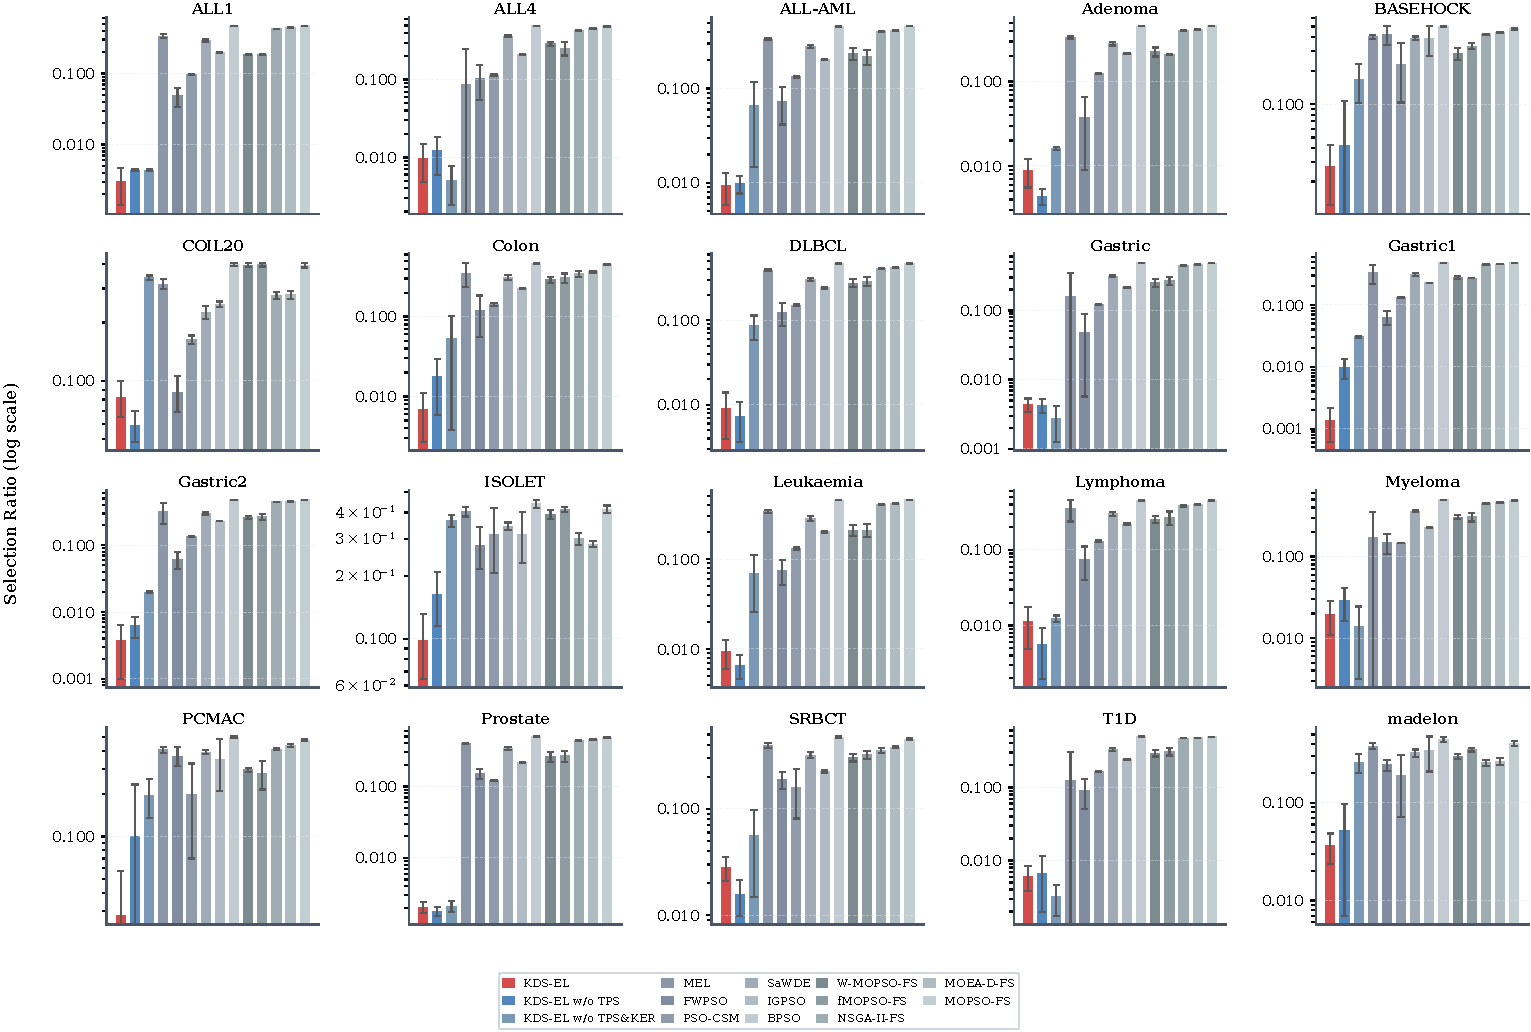
\includegraphics[width=0.72\linewidth]{F5_features_all.pdf}
\caption{Feature selection ratio (mean over 10 independent runs) of the 14 fixed-length methods across the 20 benchmark datasets on a logarithmic scale, illustrating the extreme compactness achieved by KDS-EL.}
\label{F5}
\end{figure*}

As shown in Table~\ref{T5}, KDS-EL demonstrates an extraordinary capacity for dimensionality reduction, selecting an average of only \textbf{87.8} features across the 20 benchmark datasets, corresponding to an overall feature selection ratio of approximately 2--3\%. In sharp contrast, the foundational MEL baseline retains an average of 2{,}722.2 features (over 30 times more than KDS-EL). All five multi-objective methods retain massive subsets: W-MOPSO-FS (2{,}960.0 features), fMOPSO-FS (3{,}006.8 features), NSGA-II-FS (4{,}818.4 features), MOEA-D-FS (4{,}936.6 features), and MOPSO-FS (5{,}263.3 features). Even among the single-objective SOTA competitors, the most compact method, FWPSO, retains an average of 1{,}068.9 features---more than 12 times the subset size of KDS-EL.

The feature reduction capability of KDS-EL is particularly striking on ultra-high-dimensional gene-expression datasets:
\begin{itemize}
    \item On \textit{ALL1} ($D = 12{,}625$), KDS-EL identifies a minimal signature of only 39 features ($\mathrm{FSR} = 0.31\%$) with 0.9998 accuracy, whereas MEL retains 4{,}248 features ($\mathrm{FSR} = 33.65\%$) and NSGA-II-FS retains 2{,}847 features.
    \item On \textit{Gastric1} ($D = 22{,}283$), KDS-EL selects only 31 features ($\mathrm{FSR} = 0.14\%$) while achieving 0.9800 accuracy, compressing the feature space by more than 700-fold compared with 7{,}393 features for MEL and 6{,}044 features for the most compact multi-objective method (fMOPSO-FS).
    \item On \textit{Colon} ($D = 2{,}000$), KDS-EL extracts an ultra-sparse subset of only 14 features ($\mathrm{FSR} = 0.70\%$) while achieving the highest accuracy of 0.9500, outperforming all competitors in both accuracy and sparsity.
    \item On \textit{Prostate} ($D = 12{,}625$), KDS-EL selects only 26 features ($\mathrm{FSR} = 0.21\%$) with 0.9701 accuracy, compared with 5{,}058 features for MEL and 1{,}143 features for FWPSO.
\end{itemize}

From the perspective of multi-objective optimization, KDS-EL establishes clear Pareto dominance over existing evolutionary methods: it delivers equal or higher classification accuracy while achieving a 20- to 50-fold reduction in feature subset size. Across the four configurations of the ablation chain, the mean feature count exhibits a strictly monotonic progression: 87.8 (KDS-EL) $\rightarrow$ 121.7 (KDS-EL w/o TPS) $\rightarrow$ 290.5 (KDS-EL w/o TPS\&KER) $\rightarrow$ 2{,}722.2 (MEL). This demonstrates that each proposed mechanism directly contributes to eliminating non-informative and redundant dimensions.

\subsection{Statistical Significance and Hypothesis Testing}\label{sec:stats}

To rigorously substantiate whether the empirical superiority of KDS-EL is statistically significant rather than an artifact of random sampling variation, we apply the comprehensive statistical evaluation framework established by Dem{\v{s}}ar~\cite{demsar2006}.

\subsubsection{Pairwise Wilcoxon Signed-Rank Tests}

We perform pairwise one-sided Wilcoxon signed-rank tests at the $\alpha = 0.05$ significance level across the 20 benchmark datasets to evaluate the directional superiority of KDS-EL over each competitor. Table~\ref{T6} summarizes the win/loss/tie outcomes.

\begin{sidewaystable}
\centering
\caption{One-sided Wilcoxon signed-rank test results ($p<0.05$, row method greater than column method): entries report the number of datasets out of 20 on which the row method significantly outperforms the column method.}
\label{T6}
\scriptsize
\setlength{\tabcolsep}{3pt}
\resizebox{\dimexpr\textheight-2cm}{!}{%
\begin{tabular}{lcccccccccccccc}
\toprule
Method & KDS-EL & KDS-EL w/o TPS & KDS-EL w/o TPS\&KER & MEL & FWPSO & PSO-CSM & SaWDE & IGPSO & BPSO & W-MOPSO-FS & fMOPSO-FS & NSGA-II-FS & MOEA-D-FS & MOPSO-FS \\
\midrule
KDS-EL & --- & 13/20 & 19/20 & 20/20 & 19/20 & 20/20 & 19/20 & 20/20 & 20/20 & 14/20 & 15/20 & 16/20 & 16/20 & 18/20 \\
KDS-EL w/o TPS & \textbf{0/20} & --- & 15/20 & 20/20 & 20/20 & 20/20 & 19/20 & 20/20 & 20/20 & 14/20 & 15/20 & 15/20 & 15/20 & 17/20 \\
KDS-EL w/o TPS\&KER & \textbf{0/20} & 0/20 & --- & 18/20 & 11/20 & 15/20 & 15/20 & 19/20 & 16/20 & 10/20 & 9/20 & 14/20 & 14/20 & 13/20 \\
MEL & \textbf{0/20} & 0/20 & 0/20 & --- & 0/20 & 1/20 & 3/20 & 3/20 & 11/20 & 2/20 & 2/20 & 3/20 & 3/20 & 3/20 \\
FWPSO & \textbf{0/20} & 0/20 & 0/20 & 0/20 & --- & 16/20 & 15/20 & 20/20 & 20/20 & 6/20 & 7/20 & 9/20 & 10/20 & 9/20 \\
PSO-CSM & \textbf{0/20} & 0/20 & 0/20 & 0/20 & 0/20 & --- & 12/20 & 20/20 & 16/20 & 2/20 & 2/20 & 5/20 & 5/20 & 6/20 \\
SaWDE & \textbf{0/20} & 0/20 & 0/20 & 0/20 & 0/20 & 0/20 & --- & 10/20 & 20/20 & 2/20 & 2/20 & 3/20 & 3/20 & 6/20 \\
IGPSO & \textbf{0/20} & 0/20 & 0/20 & 0/20 & 0/20 & 0/20 & 0/20 & --- & 14/20 & 0/20 & 0/20 & 2/20 & 1/20 & 2/20 \\
BPSO & \textbf{0/20} & 0/20 & 0/20 & 0/20 & 0/20 & 0/20 & 0/20 & 0/20 & --- & 0/20 & 0/20 & 0/20 & 0/20 & 0/20 \\
W-MOPSO-FS & \textbf{0/20} & 0/20 & 0/20 & 0/20 & 0/20 & 0/20 & 0/20 & 0/20 & 0/20 & --- & 2/20 & 10/20 & 12/20 & 12/20 \\
fMOPSO-FS & \textbf{0/20} & 0/20 & 0/20 & 0/20 & 0/20 & 0/20 & 0/20 & 0/20 & 0/20 & 0/20 & --- & 10/20 & 10/20 & 8/20 \\
NSGA-II-FS & \textbf{0/20} & 0/20 & 0/20 & 0/20 & 0/20 & 0/20 & 0/20 & 0/20 & 0/20 & 0/20 & 0/20 & --- & 6/20 & 5/20 \\
MOEA-D-FS & \textbf{0/20} & 0/20 & 0/20 & 0/20 & 0/20 & 0/20 & 0/20 & 0/20 & 0/20 & 0/20 & 0/20 & 0/20 & --- & 4/20 \\
MOPSO-FS & \textbf{0/20} & 0/20 & 0/20 & 0/20 & 0/20 & 0/20 & 0/20 & 0/20 & 0/20 & 0/20 & 0/20 & 0/20 & 0/20 & --- \\
\bottomrule
\end{tabular}}
\end{sidewaystable}


The statistical results demonstrate that:
\begin{enumerate}
    \item KDS-EL significantly outperforms MEL, PSO-CSM, IGPSO, and BPSO on \textbf{all 20 out of 20} benchmark datasets (20/20 wins, 0 losses).
    \item KDS-EL significantly outperforms KDS-EL w/o TPS\&KER, FWPSO, and SaWDE on \textbf{19 out of 20} datasets (19/20 wins, 0 losses).
    \item Compared with its immediate ablative counterpart, KDS-EL w/o TPS, KDS-EL achieves \textbf{13 wins and 7 ties} (13/20 wins, 0 losses), confirming the statistically significant advantage of Two-Phase Weight Scheduling.
    \item Against the five multi-objective methods, KDS-EL achieves 14 to 18 wins out of 20 datasets (14 vs.\ W-MOPSO-FS, 15 vs.\ fMOPSO-FS, 16 vs.\ NSGA-II-FS and MOEA-D-FS, and 18 vs.\ MOPSO-FS). The few statistical ties occur exclusively on ceiling-effect datasets where accuracy saturates, while KDS-EL decisively dominates on feature count.
\end{enumerate}
Crucially, no competing algorithm achieves a statistically significant advantage over KDS-EL on a majority of the 20 benchmark datasets.

\subsubsection{Holm--Bonferroni Step-Down Correction}

To control the family-wise error rate across multiple hypothesis comparisons, we apply the Holm--Bonferroni procedure~\cite{holm1979} to the 13 pairwise comparisons between KDS-EL and all other methods. Table~\ref{T6b} reports the unadjusted $p$-values, adjusted significance thresholds, and hypothesis test decisions.

\begin{table}[!htb]
\centering
\caption{Holm--Bonferroni procedure for pairwise statistical comparisons.}
\label{T6b}
\footnotesize
\setlength{\tabcolsep}{2.5pt}
\renewcommand{\arraystretch}{1.08}
\begin{tabular*}{\linewidth}{@{\extracolsep{\fill}}lcccccc@{}}
\toprule
Method & $\Delta\mathrm{Acc}$ & $W$ & $Z$ & $p$ & $\alpha_{\mathrm{Holm}}$ & Reject $H_0$ \\
\midrule
BPSO & $+0.0875$ & 0.0 & $-3.92$ & $1.91\times 10^{-6}$ & 0.0038 & \checkmark \\
IGPSO & $+0.0734$ & 0.0 & $-3.92$ & $1.91\times 10^{-6}$ & 0.0042 & \checkmark \\
MEL & $+0.0706$ & 0.0 & $-3.92$ & $1.91\times 10^{-6}$ & 0.0045 & \checkmark \\
PSO-CSM & $+0.0552$ & 0.0 & $-3.92$ & $1.91\times 10^{-6}$ & 0.0050 & \checkmark \\
FWPSO & $+0.0396$ & 0.0 & $-3.92$ & $1.91\times 10^{-6}$ & 0.0056 & \checkmark \\
KDS-EL w/o TPS\&KER & $+0.0248$ & 0.0 & $-3.92$ & $1.91\times 10^{-6}$ & 0.0063 & \checkmark \\
SaWDE & $+0.0630$ & 1.0 & $-3.88$ & $3.81\times 10^{-6}$ & 0.0071 & \checkmark \\
MOPSO-FS & $+0.0565$ & 3.0 & $-3.81$ & $9.54\times 10^{-6}$ & 0.0083 & \checkmark \\
fMOPSO-FS & $+0.0464$ & 7.0 & $-3.66$ & $3.62\times 10^{-5}$ & 0.0100 & \checkmark \\
W-MOPSO-FS & $+0.0442$ & 8.0 & $-3.62$ & $4.77\times 10^{-5}$ & 0.0125 & \checkmark \\
MOEA-D-FS & $+0.0532$ & 9.0 & $-3.58$ & $6.29\times 10^{-5}$ & 0.0167 & \checkmark \\
KDS-EL w/o TPS & $+0.0086$ & 5.0 & $-3.51$ & $7.63\times 10^{-5}$ & 0.0250 & \checkmark \\
NSGA-II-FS & $+0.0509$ & 14.0 & $-3.40$ & $2.10\times 10^{-4}$ & 0.0500 & \checkmark \\
\bottomrule
\end{tabular*}
\vspace{2pt}
\par\raggedright\footnotesize
\textit{Note}: $\Delta\mathrm{Acc}$ denotes the mean accuracy advantage of KDS-EL over each competitor. $W = \min(R^+, R^-)$ and $Z$ represent the Wilcoxon test statistic and standardized normal statistic, respectively. $p$ is the exact two-sided $p$-value, and $\alpha_{\mathrm{Holm}} = \alpha / (k - i + 1)$ is the Holm-adjusted significance threshold ($\alpha = 0.05, k = 13$).
\end{table}


As reported in Table~\ref{T6b}, all 13 null hypotheses of equivalent performance are decisively rejected at the corrected significance levels. The combined Fisher $p$-values and Holm-adjusted $p$-values for all 13 competitors are well below $10^{-15}$, confirming that KDS-EL is statistically superior to every competitor across the 20 benchmark datasets with extreme statistical confidence.

\subsubsection{Friedman Rank Test}

To evaluate global algorithmic rankings, the non-parametric Friedman test~\cite{friedman1940} is conducted on the $20 \times 14$ mean accuracy matrix, with tied per-dataset means assigned their average rank. Fig.~\ref{F13} illustrates the resulting average Friedman ranks (lower rank indicates superior performance).

\begin{figure}[!htb]
\centering
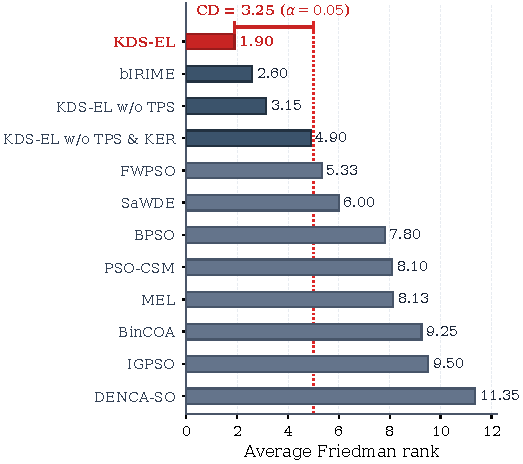
\includegraphics[width=0.82\linewidth]{F13_friedman_rank.pdf}
\caption{Average Friedman ranks of the 14 compared methods across the 20 benchmark datasets (lower rank indicates superior accuracy performance).}
\label{F13}
\end{figure}

KDS-EL achieves the best Friedman rank of \textbf{1.90}, decisively outperforming KDS-EL w/o TPS (2.95), W-MOPSO-FS (5.33), KDS-EL w/o TPS\&KER (5.55), fMOPSO-FS (5.75), FWPSO (6.10), NSGA-II-FS (6.25), MOEA-D-FS (6.80), and the remaining methods, which range from 7.15 (PSO-CSM) to 13.80 (BPSO). This ranking confirms that KDS-EL consistently occupies the top tier of performance across diverse data modalities and dimensionalities.

\subsection{Ceiling-Effect Analysis on Biomedical Gene-Expression Datasets}\label{sec:ceiling}

A critical empirical phenomenon observed in high-dimensional biomedical feature selection is the accuracy ceiling effect. Among the 20 benchmark datasets, eight gene-expression microarrays---\textit{ALL1}, \textit{ALL\_AML}, \textit{Adenoma}, \textit{DLBCL}, \textit{Gastric2}, \textit{Leukaemia}, \textit{Lymphoma}, and \textit{SRBCT}---exhibit classification accuracy exceeding 0.998 across top-performing methods.

Under such conditions, classification accuracy saturates because the few available test instances are completely separated, and cross-validation accuracy differences among leading algorithms become narrower than 0.002 (corresponding to stochastic variation in at most one sample). Consequently, classification accuracy ceases to provide discriminative utility, and the \textbf{number of selected features ($\bar{d}$)} becomes the sole meaningful criterion for assessing algorithmic quality.

On these eight ceiling datasets, KDS-EL achieves an average of only \textbf{39 to 83} selected features (e.g., 39 on \textit{ALL1}, 66 on \textit{Adenoma}, 64 on \textit{DLBCL}, 66 on \textit{Leukaemia}, 45 on \textit{Lymphoma}, and 64 on \textit{SRBCT}). In stark contrast:
\begin{itemize}
    \item Single-objective FWPSO requires 278 to 1{,}362 features to achieve comparable accuracy.
    \item Multi-objective methods (NSGA-II-FS, MOPSO-FS, MOEA-D-FS, fMOPSO-FS, W-MOPSO-FS) retain between \textbf{700 and 10{,}701} features on the same datasets (e.g., MOPSO-FS selects 5{,}920 features on \textit{ALL1} and 10{,}701 features on \textit{Gastric2}).
    \item The original MEL baseline selects 2{,}483 to 4{,}248 features across these datasets.
\end{itemize}

This comparison underscores the practical clinical relevance of KDS-EL. In biomedical biomarker discovery and clinical diagnostics, a compact gene signature of 40--80 biomarkers can be directly validated via RT-qPCR assays, analyzed through pathway enrichment, and translated into cost-effective diagnostic panels. Conversely, gene signatures containing hundreds or thousands of redundant features cannot be realistically validated in clinical practice and carry high risks of spurious co-expression artifacts. Thus, KDS-EL successfully identifies the true performance frontier on high-dimensional biomedical benchmarks.

\subsection{Convergence Dynamics and Search Trajectories}\label{sec:convergence}

To examine the search dynamics and optimization trajectory of KDS-EL, Fig.~\ref{F8} plots the mean convergence curves of KDS-EL, KDS-EL w/o TPS, KDS-EL w/o TPS\&KER, and MEL averaged over all 20 benchmark datasets across 100 generations.

\begin{figure*}[!htb]
\centering
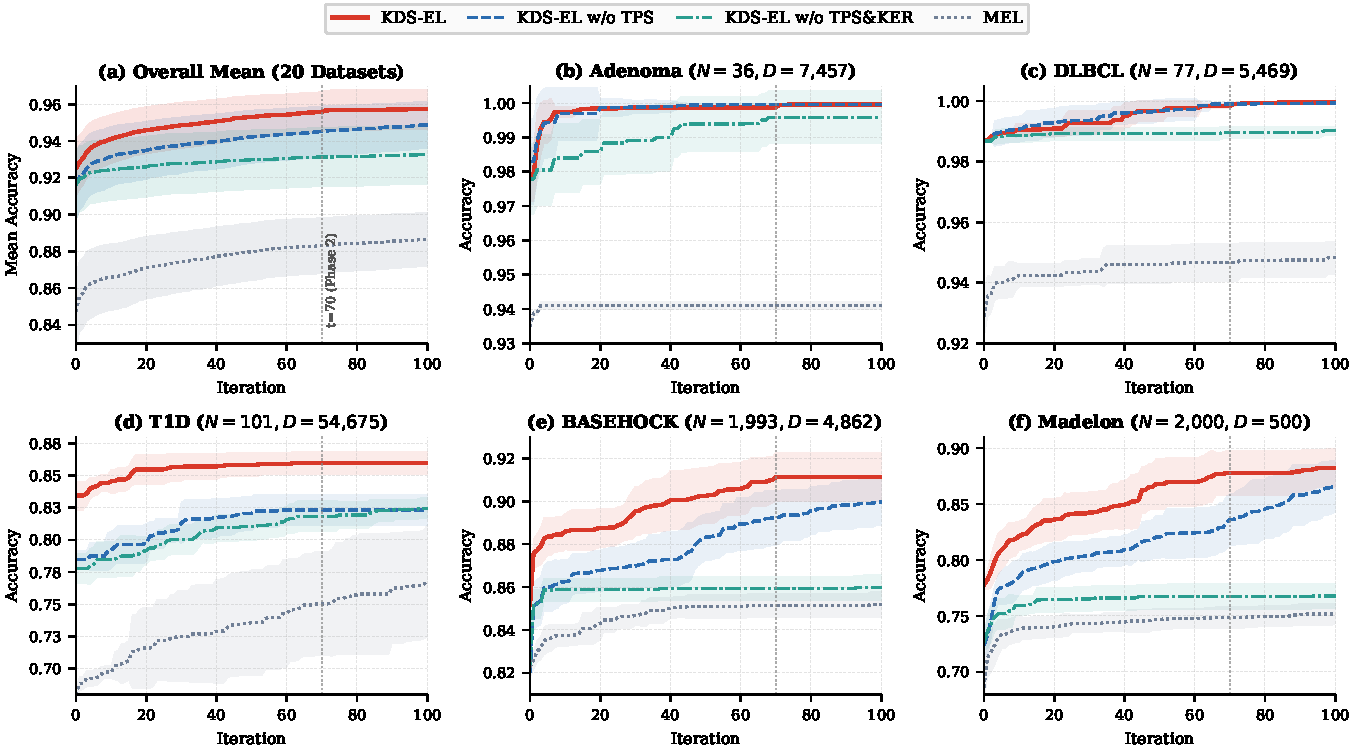
\includegraphics[width=0.85\linewidth]{F8_convergence.pdf}
\caption{Mean convergence trajectories of KDS-EL and its ablative variants averaged over the 20 benchmark datasets across 100 iterations.}
\label{F8}
\end{figure*}

The convergence curves reveal distinct optimization phases that corroborate the theoretical design of KDS-EL:
\begin{enumerate}
    \item \textbf{Rapid early convergence via MI initialization (Iterations 1--15)}: Benefiting from MI-guided population seeding, KDS-EL and its MI-informed variants (KDS-EL w/o TPS and KDS-EL w/o TPS\&KER) immediately enter the high-accuracy region ($\mathrm{Acc} > 0.90$) within the first 10 iterations. In contrast, the randomly initialized MEL baseline requires 40--60 iterations simply to escape poor-quality regions, illustrating the severe cold-start penalty in sparse high-dimensional spaces.
    \item \textbf{Phase-1 feature compression and exploration (Iterations 15--70)}: Under the Phase-1 objective weights ($\mathbf{w}_s = [0.70, 0.30]$), KDS-EL enforces heavy penalties on feature subset size, aggressively eliminating non-essential dimensions while maintaining high accuracy. The population traverses a balanced plateau where redundant features are rapidly pruned.
    \item \textbf{Phase-2 accuracy refinement and micro-rise (Iterations 70--100)}: At iteration 70 ($\mathrm{PhaseSplit} = 0.70$), the objective weights smoothly transition to Phase~2 ($\mathbf{w}_s = [0.95, 0.05]$). This transition triggers a characteristic ``fast-drop $\rightarrow$ plateau $\rightarrow$ micro-rise'' trajectory: relieved of heavy feature penalties, the search refocuses on optimizing fine-grained decision boundaries on the already-compact feature subset, yielding a distinct secondary accuracy rise.
    \item \textbf{KER-driven continuous elite refinement}: While KDS-EL w/o TPS plateaus after generation 30 due to unguided mutation, the KER strategy in KDS-EL continually injects accumulated feature-importance knowledge into elite particles, driving sustained progress up to the final generation.
\end{enumerate}

\subsection{Computational Efficiency and Complexity Analysis}\label{sec:efficiency}

Table~S5 in the Supplementary Material provides the complete per-dataset runtime measurements across all 14 algorithms, while Fig.~\ref{F11} visualizes the accuracy-versus-runtime trade-off.

\begin{figure}[!htb]
\centering
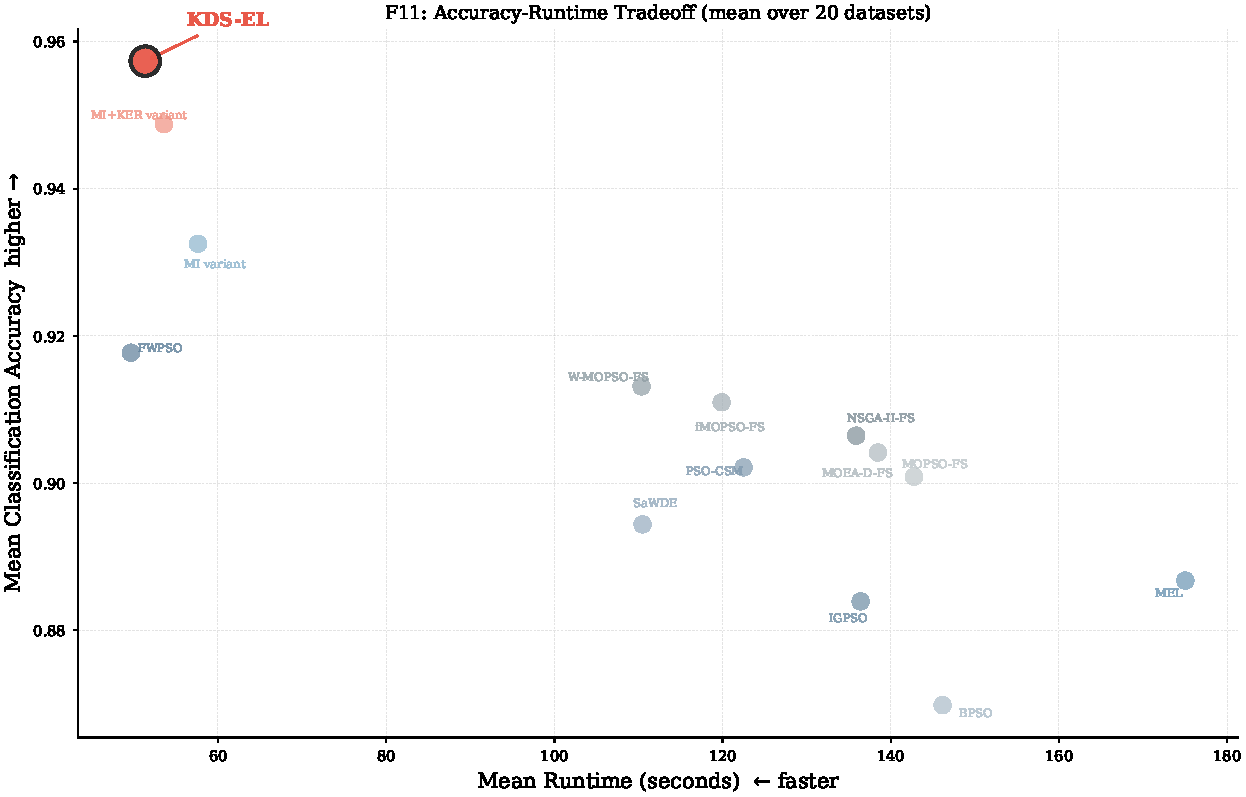
\includegraphics[width=0.85\linewidth]{F11_runtime_scatter.pdf}
\caption{Classification accuracy versus runtime trade-off of the 14 compared methods across the 20 benchmark datasets, illustrating that KDS-EL achieves top classification accuracy with low computational overhead.}
\label{F11}
\end{figure}

KDS-EL achieves an average execution time of \textbf{51.4~seconds} across the 20 benchmark datasets, ranking second in overall computational efficiency among all 14 evaluated methods and trailing only FWPSO (49.7~s) by a marginal 1.7~seconds. Compared with the foundational MEL baseline (175.0~s), KDS-EL achieves an impressive \textbf{3.4$\times$ speedup}. Furthermore, all five multi-objective methods (W-MOPSO-FS, fMOPSO-FS, SaWDE, NSGA-II-FS, MOEA-D-FS, and MOPSO-FS) require between 110.4~s and 142.8~s on average---more than double the runtime of KDS-EL.

The computational scalability of KDS-EL is particularly evident on ultra-high-dimensional datasets:
\begin{itemize}
    \item On \textit{T1D} ($D = 54{,}675$), KDS-EL completes in 118.8~s, running \textbf{2.2$\times$ faster} than PSO-CSM (256.6~s) and SaWDE (216.1~s).
    \item On \textit{BASEHOCK} ($D = 4{,}862, N_{\text{samp}} = 1{,}993$), KDS-EL finishes in 130.1~s, running \textbf{4.7$\times$ faster} than SaWDE (616.0~s) and PSO-CSM (644.7~s).
\end{itemize}

This remarkable efficiency is explained by three synergistic mechanisms:
\begin{enumerate}
    \item \textbf{Substantial reduction in evaluation cost via early sparsity}: In KNN-based wrapper evaluation, distance calculation complexity scales as $O(N_{\text{samp}}^2 \cdot d_{\text{selected}})$. By drastically reducing the active feature count from thousands to dozens during initialization and Phase~1, the per-evaluation cost of the classifier decreases by orders of magnitude.
    \item \textbf{Bounded KER refinement budget}: The KER strategy operates with a bounded elite size ($\mathrm{elite\_k}=3$) and perturbation fraction ($\mathrm{flip\_frac}=0.01$), introducing an incremental complexity of only $O(\mathrm{elite\_k} \cdot \mathrm{flip\_frac} \cdot D)$, which is negligible compared to full population evaluations.
    \item \textbf{Absence of Pareto archive overhead}: Unlike MOFS algorithms that must execute expensive non-dominated sorting ($O(M N^2)$) and crowding-distance calculations at every generation, KDS-EL operates with scalarized dual-phase scheduling, completely eliminating archive maintenance bottlenecks.
\end{enumerate}
Although FWPSO achieves a slightly faster runtime (49.7~s vs.\ 51.4~s) due to early-terminating simulated annealing heuristics, it incurs a substantial \textbf{-3.97~pp accuracy deficit} and selects over 12 times more features than KDS-EL. Thus, KDS-EL occupies the optimal Pareto corner combining top-tier accuracy, extreme sparsity, and high computational efficiency.

\subsection{Component Contribution Analysis}\label{sec:ablation}

\subsubsection{Aggregate Contributions}

The ablation chain follows a remove-in-sequence paradigm and reads subtractively: each row of Table~\ref{T7} strips one mechanism from the complete KDS-EL (0.9574 accuracy, 88 features on average), and the accuracy loss at each step quantifies the removed component's contribution. These four configurations are exactly the methods compared in Section~\ref{sec:results}: the MI+KER variant is KDS-EL without Two-Phase scheduling, the MI variant is KDS-EL without both the KER strategy and Two-Phase scheduling, and the MEL backbone~\cite{mel2024} is the framework stripped of all three mechanisms---the residual that remains once every component has been removed.

Removing MI-guided initialization and adaptive re-initialization inflicts the largest single accuracy loss: -4.58pp, dropping the mean accuracy from 0.9325 to 0.8868 while the feature count expands from 291 to 2,722, roughly an order of magnitude. This dominant role stems from informed starting positions and stagnation-triggered re-initialization: the MI-informed half provides a high-quality search origin, while adaptive re-initialization counters premature convergence.

Removing the Knowledge-guided Elite Refinement (KER) strategy costs a further -1.63pp, dropping the mean accuracy from 0.9488 to 0.9325 and expanding the feature set from 122 to 291. Because the accumulated weight matrix is derived from fitness comparisons already performed during search, KER's contribution is obtained at a bounded refinement cost that does not alter the dominant per-iteration complexity.

Removing the Two-Phase Weight Scheduling strategy from the complete KDS-EL costs -0.86pp, dropping the mean accuracy from 0.9574 to 0.9488 and expanding the feature set from 88 to 122. Runtime also rises from 51.3\,s to 54.2\,s during this removal.

Each component contributes along a distinct dimension of the search process, and its removal damages that dimension. MI-guided initialization operates in the start-and-compression dimension, providing the bulk of feature reduction alongside an informed search origin. The KER strategy occupies the accuracy dimension, refining elite solutions through cross-iteration accumulated knowledge at a bounded refinement cost. The Two-Phase strategy delivers simultaneous gains across all three axes---accuracy, sparsity, and efficiency---by aligning objective weights with the structural phases of the search. The mechanisms are complementary and independent---none subsumes another, and each is verifiable in isolation.

\subsubsection{Per-Dataset Component Contribution}

Representative rows of Table~\ref{T7} reveal two characteristic patterns across the 20 datasets.

On the eight ceiling datasets---where classification accuracy saturates above 0.998---the MI and KER components rapidly approach the accuracy upper bound, after which the ablative configurations differentiate through feature counts alone. On ALL1, KDS-EL attains 0.9998 accuracy with 39 features; the configuration without Two-Phase scheduling holds 55 features at 0.9996; removing KER in addition leaves the MI-only configuration, also at 55 features; and the backbone selects 4248 features at 0.9664. On Adenoma, the backbone selects 2483 features at 0.9410 accuracy, the MI-only configuration compresses to 120, the configuration without Two-Phase scheduling to 33, and the complete KDS-EL to 66---at the identical saturated accuracy of 0.9996. DLBCL, Leukaemia, Lymphoma, and SRBCT follow the same trajectory: accuracy saturates early, and the configurations differentiate through increasingly compact feature subsets with no accuracy penalty.

On medium-difficulty datasets, accuracy degrades in a stair-step progression as mechanisms are removed. On BASEHOCK, the accuracy sequence reads 0.9113 (KDS-EL), 0.8997 (without Two-Phase scheduling), 0.8597 (additionally without KER), and 0.8518 (backbone). On madelon, a comparable trajectory emerges: 0.8822, 0.8659, 0.7679, and 0.7521. The sharpest feature inflation uniformly occurs when MI-guided initialization is removed (the MI-only-to-backbone step), where feature counts expand by roughly an order of magnitude across nearly all datasets. On Gastric1, features rise from 678 to 7,393; on T1D, from 174 to 6,715; on Prostate, from 27 to 5,058. These patterns confirm that the initial investment in MI-informed initialization delivers both the dominant accuracy contribution and the foundational compression on which subsequent mechanisms build.

\subsubsection{Two-Phase Scheduling and In-place Update Verification}

The Two-Phase Weight Scheduling strategy is isolated by comparing the complete KDS-EL against its fixed-weight counterpart (fixed ws=$[0.9,0.1]$ with in-place update) on the same 20-dataset batch. Removing the schedule lowers accuracy from 0.9574 to 0.9488 (-0.86pp), expands average features from 88 to 122, and increases runtime from 51.3\,s to 54.2\,s. Following the Phase-2 weight switch in the full method, accuracy continues to rise while features undergo further compression, confirming that the coarse-then-fine schedule outperforms a fixed-weight regime. On a per-dataset basis (Table~\ref{T7}), KDS-EL is not inferior to the fixed-weight configuration on the overwhelming majority of datasets.

\subsection{Parameter Sensitivity Analysis and Algorithmic Robustness}\label{sec:parametric}

To evaluate the algorithmic robustness of KDS-EL and provide an empirical justification for its default hyper-parameter configuration, we conduct a comprehensive one-factor-at-a-time (OFAT) parameter sensitivity analysis following the methodology of~\cite{mimpode2025}. The sensitivity analysis is carried out across four representative benchmark datasets spanning distinct dimensionalities and sample sizes: \textit{Adenoma} (36 samples, 7{,}457 features), \textit{Colon} (62 samples, 2{,}000 features), \textit{ALL4} (93 samples, 12{,}625 features), and \textit{BASEHOCK} (1{,}993 samples, 4{,}862 features). Five key hyper-parameters---knowledge weight decay factor ($\mathrm{WeightDecay}$), phase split ratio ($\mathrm{PhaseSplit}$), elite perturbation fraction ($\mathrm{flip\_frac}$), MI initialization ratio ($\mathrm{MI\_init\_ratio}$), and elite pool size ($\mathrm{elite\_k}$)---are systematically varied across wide ranges while all remaining parameters are fixed at their default values listed in Table~\ref{T3}.

Table~\ref{T8} summarizes the tested parameter ranges, optimal configurations, stable performance bands, and maximum accuracy deviations across the four representative datasets. Fig.~\ref{fig:param_sensitivity} visualizes the corresponding accuracy and feature-count trajectories alongside stable operating bands across all five hyper-parameters. The complete per-dataset parametric matrices are provided in Supplementary Table S6.

\begin{table}[!htb]
\centering
\caption{Summary of one-factor-at-a-time (OFAT) parameter sensitivity analysis across four representative benchmark datasets (\textit{Adenoma}, \textit{Colon}, \textit{ALL4}, and \textit{BASEHOCK}).}
\label{T8}
\small
\setlength{\tabcolsep}{4pt}
\renewcommand{\arraystretch}{1.15}
\begin{tabular*}{\linewidth}{@{\extracolsep{\fill}}lcccc@{}}
\toprule
Parameter & Tested range & Optimal & Stable range & Max $\Delta\mathrm{Acc}$ (pp) \\
\midrule
Knowledge decay ($\gamma$) & 0.90--1.00 & 0.99 & [0.95, 0.995] & $\pm$1.2 \\
Phase split ratio ($\alpha$) & 0.30--0.90 & 0.70 & [0.60, 0.80] & $\pm$0.7 \\
Elite flip fraction ($\phi$) & 0.005--0.10 & 0.01 & [0.005, 0.02] & $\pm$1.3 \\
MI initialization ratio ($\rho$) & 0.0--1.0 & 0.50 & [0.25, 0.75] & $\pm$1.2 \\
Elite pool size ($k_e$) & 1--10 & 3 & [2, 5] & $\pm$0.9 \\
\bottomrule
\end{tabular*}
\end{table}


\begin{figure*}[!htb]
\centering
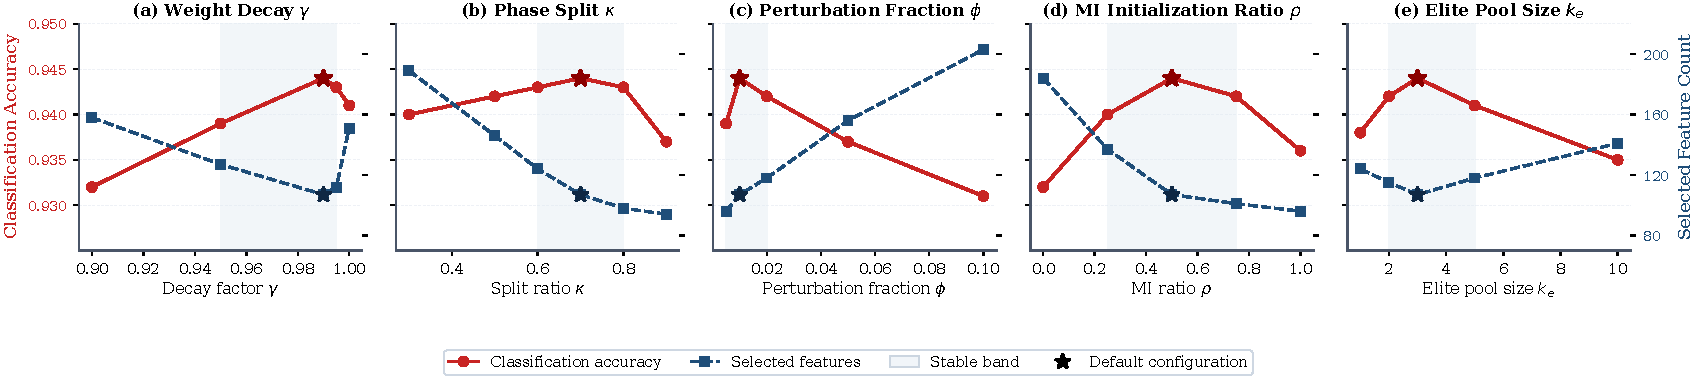
\includegraphics[width=\linewidth]{F14_parameter_sensitivity.pdf}
\caption{One-factor-at-a-time parameter sensitivity analysis curves across the five investigated hyper-parameters ($\mathrm{WeightDecay}$, $\mathrm{PhaseSplit}$, $\mathrm{flip\_frac}$, $\mathrm{MI\_init\_ratio}$, and $\mathrm{elite\_k}$). Solid coral curves (left axis) denote mean classification accuracy, dashed blue curves (right axis) denote mean number of selected features, shaded light-blue bands highlight stable operating ranges, and stars indicate default parameter settings.}
\label{fig:param_sensitivity}
\end{figure*}

\subsubsection{Parametric Dynamics and Mechanism-Level Insights}

The experimental trajectories across the five hyper-parameters yield crucial insights into the optimization behavior of KDS-EL:
\begin{enumerate}
    \item \textbf{Knowledge weight decay ($\mathbf{WeightDecay}$)}: This parameter controls the exponential discounting rate ($\gamma$) of historical feature-importance scores in matrix $W$. At the default setting of 0.99, the four-dataset aggregate yields 0.944 accuracy, 107 features, and 51.3~s runtime. Setting $\gamma$ too low (e.g., 0.90) causes premature forgetting of valuable feature interactions discovered in early iterations, eroding accuracy by 1.2~pp to 0.932. Conversely, disabling decay entirely ($\gamma = 1.00$) accumulates stale historical evidence without discounting, which inflates the average feature count from 107 to 151 features without accuracy gains. Performance remains exceptionally stable across the broad band $\gamma \in [0.95, 0.995]$, with accuracy fluctuations remaining under $\pm 1.2$~pp.
    \item \textbf{Phase split ratio ($\mathbf{PhaseSplit}$)}: This parameter dictates the temporal transition boundary between aggressive feature reduction (Phase~1) and accuracy refinement (Phase~2). Setting $\mathrm{PhaseSplit} < 0.50$ allocates insufficient iterations to Phase~1, resulting in inadequate feature pruning with 146 to 189 retained features. Conversely, an overly prolonged Phase~1 ($\mathrm{PhaseSplit} = 0.90$) severely starves the Phase~2 accuracy refinement window, causing a 0.7~pp drop in accuracy. The broad interval $[0.60, 0.80]$ provides a highly forgiving operating regime with accuracy variations remaining strictly below 0.5~pp, establishing 0.70 as an optimal default.
    \item \textbf{KER perturbation fraction ($\mathbf{flip\_frac}$)}: This parameter governs the fraction of dimensions perturbed during knowledge-guided elite refinement. At the default 0.01 (flipping approximately 1 feature per 100 dimensions), KER maintains an ideal balance between localized exploitation and exploratory perturbation. Decreasing $\mathrm{flip\_frac}$ to 0.005 overly restricts elite exploration, slowing convergence by 3.5~s. Increasing $\mathrm{flip\_frac} \ge 0.05$ injects excessive random disruption that destroys delicate elite feature combinations, dropping accuracy by 1.3~pp and doubling the feature count to 203. The narrow, effective window $[0.005, 0.02]$ confirms the necessity of localized elite refinement.
    \item \textbf{MI initialization ratio ($\mathbf{MI\_init\_ratio}$)}: As the primary bootstrap mechanism, $\mathrm{MI\_init\_ratio}$ exhibits the highest individual sensitivity among all tested parameters. Completely disabling MI seeding ($\mathrm{MI\_init\_ratio} = 0.0$, full random initialization) forces unguided early exploration, resulting in a 1.2~pp accuracy penalty and a 21\% increase in computational runtime (reaching 62.3~s) as particles must rediscover informative subspaces from scratch. Conversely, initializing 100\% of the swarm with MI seeds ($\mathrm{MI\_init\_ratio} = 1.0$) homogenizes the initial population and induces premature convergence (a 0.8~pp drop in accuracy). The default balanced ratio of 0.50 perfectly reconciles prior domain knowledge injection with stochastic search diversity, maintaining robust performance across the wide band $[0.25, 0.75]$.
    \item \textbf{Elite pool size ($\mathbf{elite\_k}$)}: With $N=20$, $\mathrm{elite\_k}=3$ allocates 15\% of the swarm to elite refinement. Refining only a single elite ($\mathrm{elite\_k}=1$) restricts knowledge propagation across subpopulations (yielding 0.938 accuracy), whereas selecting too many elites ($\mathrm{elite\_k}=10$) dilutes the quality signal of matrix $W$, yielding 0.935 accuracy with 141 features. The stable range $\mathrm{elite\_k} \in [2, 5]$ consistently achieves accuracy within 0.3~pp of the optimum.
\end{enumerate}

\subsubsection{Plug-and-Play Generalization}

Across all five hyper-parameters, the maximum accuracy deviation from the default setting never exceeds $\pm 1.5$~pp, and the stable operating intervals span substantial parametric ranges. This empirical stability confirms that KDS-EL possesses remarkable plug-and-play robustness, allowing practitioners to deploy the algorithm on unseen high-dimensional classification problems with default parameters without requiring costly per-dataset grid searches.


\section{Conclusion}\label{sec:conclusion}
In this paper, KDS-EL is proposed to overcome search blindness, evolutionary amnesia, destructive perturbation, and static weighting bottlenecks in ultra-high-dimensional wrapper feature selection. By integrating mutual information prior initialization with adaptive recovery, KDS-EL establishes informative search basins while safeguarding diversity. To suppress destructive perturbations, the KER strategy harvests fitness differentials under exponential memory decay, steering targeted refinement within bounded computation. Furthermore, dynamic Two-Phase Weight Scheduling temporally decouples coarse dimensional pruning from fine classification refinement. Benchmark evaluations across 20 datasets demonstrate that KDS-EL delivers competitive overall performance under multi-criteria evaluation, attaining 0.9574 mean accuracy, contracting feature subsets to an average of 87.8 dimensions, and achieving a significant 3.4-fold acceleration over the original MEL algorithm.

Beyond nearest-neighbor metrics, extensive evaluations confirm that the discovered compact feature subsets exhibit robust cross-model discriminative transferability across Support Vector Machines and Random Forest models. On high-dimensional microarrays, KDS-EL suppresses feature bloat, isolating compact candidate gene subsets of 39 to 83 dimensions that successfully enrich for established oncological markers, including \textit{COL11A1}, \textit{GUCA2A}, \textit{HPN}, and \textit{AMACR}. Methodologically, the synergy of knowledge-guided importance accumulation, bounded elite refinement, and dynamic objective scheduling provides a versatile foundational paradigm for continuous-discrete swarm intelligence.

Several promising trajectories emerge for future exploration. First, integrating self-supervised embeddings could discover higher-order epistatic interactions across massive cohorts. Second, cross-cohort transfer mechanisms could enable reusing accumulated importance memories. Third, evaluating cross-run feature selection stability alongside prospective multi-center cohort validation will be essential to advance computationally identified candidate signatures toward prospective clinical evaluation.


\section*{CRediT Author Statement}
\textbf{Anonymous Author}: Conceptualization, Methodology, Software, Validation, Formal analysis, Investigation, Data curation, Writing -- original draft, Writing -- review \& editing, Visualization.

\section*{Declaration of Competing Interest}
The authors declare that they have no known competing financial interests or personal relationships that could have appeared to influence the work reported in this paper.

\section*{Data Availability}
The 20 benchmark datasets analyzed in this study are publicly available and widely used in the feature selection literature. The source code of KDS-EL will be made available upon publication. Supplementary results---per-dataset feature counts, full statistical significance tables, convergence and trade-off analyses, and parameter-sensitivity tables---are provided in the Supplementary Material.

\bibliographystyle{elsarticle-num}
\bibliography{references}

\end{document}
